% Options for packages loaded elsewhere
\PassOptionsToPackage{unicode}{hyperref}
\PassOptionsToPackage{hyphens}{url}
\PassOptionsToPackage{dvipsnames,svgnames,x11names}{xcolor}
%
\documentclass[
  12pt,
  a4paper,
  DIV=11,
  numbers=noendperiod]{scrartcl}

\usepackage{amsmath,amssymb}
\usepackage{lmodern}
\usepackage{setspace}
\usepackage{iftex}
\ifPDFTeX
  \usepackage[T1]{fontenc}
  \usepackage[utf8]{inputenc}
  \usepackage{textcomp} % provide euro and other symbols
\else % if luatex or xetex
  \usepackage{unicode-math}
  \defaultfontfeatures{Scale=MatchLowercase}
  \defaultfontfeatures[\rmfamily]{Ligatures=TeX,Scale=1}
\fi
% Use upquote if available, for straight quotes in verbatim environments
\IfFileExists{upquote.sty}{\usepackage{upquote}}{}
\IfFileExists{microtype.sty}{% use microtype if available
  \usepackage[]{microtype}
  \UseMicrotypeSet[protrusion]{basicmath} % disable protrusion for tt fonts
}{}
\makeatletter
\@ifundefined{KOMAClassName}{% if non-KOMA class
  \IfFileExists{parskip.sty}{%
    \usepackage{parskip}
  }{% else
    \setlength{\parindent}{0pt}
    \setlength{\parskip}{6pt plus 2pt minus 1pt}}
}{% if KOMA class
  \KOMAoptions{parskip=half}}
\makeatother
\usepackage{xcolor}
\usepackage[top=30mm,left=20mm,right=20mm,bottom=30mm,heightrounded]{geometry}
\setlength{\emergencystretch}{3em} % prevent overfull lines
\setcounter{secnumdepth}{5}
% Make \paragraph and \subparagraph free-standing
\ifx\paragraph\undefined\else
  \let\oldparagraph\paragraph
  \renewcommand{\paragraph}[1]{\oldparagraph{#1}\mbox{}}
\fi
\ifx\subparagraph\undefined\else
  \let\oldsubparagraph\subparagraph
  \renewcommand{\subparagraph}[1]{\oldsubparagraph{#1}\mbox{}}
\fi

\usepackage{color}
\usepackage{fancyvrb}
\newcommand{\VerbBar}{|}
\newcommand{\VERB}{\Verb[commandchars=\\\{\}]}
\DefineVerbatimEnvironment{Highlighting}{Verbatim}{commandchars=\\\{\}}
% Add ',fontsize=\small' for more characters per line
\usepackage{framed}
\definecolor{shadecolor}{RGB}{241,243,245}
\newenvironment{Shaded}{\begin{snugshade}}{\end{snugshade}}
\newcommand{\AlertTok}[1]{\textcolor[rgb]{0.68,0.00,0.00}{#1}}
\newcommand{\AnnotationTok}[1]{\textcolor[rgb]{0.37,0.37,0.37}{#1}}
\newcommand{\AttributeTok}[1]{\textcolor[rgb]{0.40,0.45,0.13}{#1}}
\newcommand{\BaseNTok}[1]{\textcolor[rgb]{0.68,0.00,0.00}{#1}}
\newcommand{\BuiltInTok}[1]{\textcolor[rgb]{0.00,0.23,0.31}{#1}}
\newcommand{\CharTok}[1]{\textcolor[rgb]{0.13,0.47,0.30}{#1}}
\newcommand{\CommentTok}[1]{\textcolor[rgb]{0.37,0.37,0.37}{#1}}
\newcommand{\CommentVarTok}[1]{\textcolor[rgb]{0.37,0.37,0.37}{\textit{#1}}}
\newcommand{\ConstantTok}[1]{\textcolor[rgb]{0.56,0.35,0.01}{#1}}
\newcommand{\ControlFlowTok}[1]{\textcolor[rgb]{0.00,0.23,0.31}{#1}}
\newcommand{\DataTypeTok}[1]{\textcolor[rgb]{0.68,0.00,0.00}{#1}}
\newcommand{\DecValTok}[1]{\textcolor[rgb]{0.68,0.00,0.00}{#1}}
\newcommand{\DocumentationTok}[1]{\textcolor[rgb]{0.37,0.37,0.37}{\textit{#1}}}
\newcommand{\ErrorTok}[1]{\textcolor[rgb]{0.68,0.00,0.00}{#1}}
\newcommand{\ExtensionTok}[1]{\textcolor[rgb]{0.00,0.23,0.31}{#1}}
\newcommand{\FloatTok}[1]{\textcolor[rgb]{0.68,0.00,0.00}{#1}}
\newcommand{\FunctionTok}[1]{\textcolor[rgb]{0.28,0.35,0.67}{#1}}
\newcommand{\ImportTok}[1]{\textcolor[rgb]{0.00,0.46,0.62}{#1}}
\newcommand{\InformationTok}[1]{\textcolor[rgb]{0.37,0.37,0.37}{#1}}
\newcommand{\KeywordTok}[1]{\textcolor[rgb]{0.00,0.23,0.31}{#1}}
\newcommand{\NormalTok}[1]{\textcolor[rgb]{0.00,0.23,0.31}{#1}}
\newcommand{\OperatorTok}[1]{\textcolor[rgb]{0.37,0.37,0.37}{#1}}
\newcommand{\OtherTok}[1]{\textcolor[rgb]{0.00,0.23,0.31}{#1}}
\newcommand{\PreprocessorTok}[1]{\textcolor[rgb]{0.68,0.00,0.00}{#1}}
\newcommand{\RegionMarkerTok}[1]{\textcolor[rgb]{0.00,0.23,0.31}{#1}}
\newcommand{\SpecialCharTok}[1]{\textcolor[rgb]{0.37,0.37,0.37}{#1}}
\newcommand{\SpecialStringTok}[1]{\textcolor[rgb]{0.13,0.47,0.30}{#1}}
\newcommand{\StringTok}[1]{\textcolor[rgb]{0.13,0.47,0.30}{#1}}
\newcommand{\VariableTok}[1]{\textcolor[rgb]{0.07,0.07,0.07}{#1}}
\newcommand{\VerbatimStringTok}[1]{\textcolor[rgb]{0.13,0.47,0.30}{#1}}
\newcommand{\WarningTok}[1]{\textcolor[rgb]{0.37,0.37,0.37}{\textit{#1}}}

\providecommand{\tightlist}{%
  \setlength{\itemsep}{0pt}\setlength{\parskip}{0pt}}\usepackage{longtable,booktabs,array}
\usepackage{calc} % for calculating minipage widths
% Correct order of tables after \paragraph or \subparagraph
\usepackage{etoolbox}
\makeatletter
\patchcmd\longtable{\par}{\if@noskipsec\mbox{}\fi\par}{}{}
\makeatother
% Allow footnotes in longtable head/foot
\IfFileExists{footnotehyper.sty}{\usepackage{footnotehyper}}{\usepackage{footnote}}
\makesavenoteenv{longtable}
\usepackage{graphicx}
\makeatletter
\def\maxwidth{\ifdim\Gin@nat@width>\linewidth\linewidth\else\Gin@nat@width\fi}
\def\maxheight{\ifdim\Gin@nat@height>\textheight\textheight\else\Gin@nat@height\fi}
\makeatother
% Scale images if necessary, so that they will not overflow the page
% margins by default, and it is still possible to overwrite the defaults
% using explicit options in \includegraphics[width, height, ...]{}
\setkeys{Gin}{width=\maxwidth,height=\maxheight,keepaspectratio}
% Set default figure placement to htbp
\makeatletter
\def\fps@figure{htbp}
\makeatother

\usepackage{booktabs}
\usepackage{longtable}
\usepackage{array}
\usepackage{multirow}
\usepackage{wrapfig}
\usepackage{float}
\usepackage{colortbl}
\usepackage{pdflscape}
\usepackage{tabu}
\usepackage{threeparttable}
\usepackage{threeparttablex}
\usepackage[normalem]{ulem}
\usepackage{makecell}
\usepackage{xcolor}
\KOMAoption{captions}{tableheading}
\usepackage[none]{hyphenat} \usepackage[danish]{babel} \usepackage{dcolumn} \usepackage{threeparttable} \usepackage{fancyhdr}
\makeatletter
\makeatother
\makeatletter
\makeatother
\makeatletter
\@ifpackageloaded{caption}{}{\usepackage{caption}}
\AtBeginDocument{%
\ifdefined\contentsname
  \renewcommand*\contentsname{Table of contents}
\else
  \newcommand\contentsname{Table of contents}
\fi
\ifdefined\listfigurename
  \renewcommand*\listfigurename{List of Figures}
\else
  \newcommand\listfigurename{List of Figures}
\fi
\ifdefined\listtablename
  \renewcommand*\listtablename{List of Tables}
\else
  \newcommand\listtablename{List of Tables}
\fi
\ifdefined\figurename
  \renewcommand*\figurename{Figure}
\else
  \newcommand\figurename{Figure}
\fi
\ifdefined\tablename
  \renewcommand*\tablename{Table}
\else
  \newcommand\tablename{Table}
\fi
}
\@ifpackageloaded{float}{}{\usepackage{float}}
\floatstyle{ruled}
\@ifundefined{c@chapter}{\newfloat{codelisting}{h}{lop}}{\newfloat{codelisting}{h}{lop}[chapter]}
\floatname{codelisting}{Listing}
\newcommand*\listoflistings{\listof{codelisting}{List of Listings}}
\makeatother
\makeatletter
\@ifpackageloaded{caption}{}{\usepackage{caption}}
\@ifpackageloaded{subcaption}{}{\usepackage{subcaption}}
\makeatother
\makeatletter
\@ifpackageloaded{tcolorbox}{}{\usepackage[many]{tcolorbox}}
\makeatother
\makeatletter
\@ifundefined{shadecolor}{\definecolor{shadecolor}{rgb}{.97, .97, .97}}
\makeatother
\makeatletter
\makeatother
\ifLuaTeX
  \usepackage{selnolig}  % disable illegal ligatures
\fi
\IfFileExists{bookmark.sty}{\usepackage{bookmark}}{\usepackage{hyperref}}
\IfFileExists{xurl.sty}{\usepackage{xurl}}{} % add URL line breaks if available
\urlstyle{same} % disable monospaced font for URLs
\hypersetup{
  pdftitle={Projekt hos Thise Mejeri},
  pdfauthor={Kenneth Gottfredsen, Eva Rauff og Sanne Sørensen},
  colorlinks=true,
  linkcolor={blue},
  filecolor={Maroon},
  citecolor={Blue},
  urlcolor={Blue},
  pdfcreator={LaTeX via pandoc}}

\title{Projekt hos Thise Mejeri}
\usepackage{etoolbox}
\makeatletter
\providecommand{\subtitle}[1]{% add subtitle to \maketitle
  \apptocmd{\@title}{\par {\large #1 \par}}{}{}
}
\makeatother
\subtitle{Et datamodenhedsprojekt der undersøger sammenhængen mellem
vejret og efterspørgslen på koldskål}
\author{Kenneth Gottfredsen, Eva Rauff og Sanne Sørensen}
\date{Dato: 5/1/23. Vejledere: Bjarne Taulo, Claus Bang \& Anna Hald.
Antal tegn: 27.496}

\begin{document}
\maketitle
\ifdefined\Shaded\renewenvironment{Shaded}{\begin{tcolorbox}[interior hidden, frame hidden, sharp corners, borderline west={3pt}{0pt}{shadecolor}, boxrule=0pt, breakable, enhanced]}{\end{tcolorbox}}\fi

\renewcommand*\contentsname{Indholdsfortegnelse}
{
\hypersetup{linkcolor=}
\setcounter{tocdepth}{3}
\tableofcontents
}
\setstretch{1.5}
\setcounter{page}{1} 
\parindent 0ex
\emergencystretch 3em
\pagestyle{fancy}
\fancyhead{}
\fancyfoot{}
\fancyfoot[C]{\thepage}
\renewcommand{\headrulewidth}{0.5pt}
\renewcommand{\footrulewidth}{0.5pt}

\hypertarget{problemfelt}{%
\section{Problemfelt}\label{problemfelt}}

Det er vanskeligt at forudsige hvor meget koldskål Thise Mejeri skal
producere til deres kunder (Kjer 2022). Sommervejret påvirker kundernes
efterspørgsel på koldskål (Holland 2022). Hos Thise Mejeri bruger
medarbejderne vejrudsigten, og mange års erfaring når de skal vurdere,
hvor mange ltr. koldskål, der skal produceres (Jensen 2022). I en
artikel fra TV Midtvest fortæller adm. direktør Poul Pedersen fra Thise
Mejeri at: \emph{``Vi kigger på tal og vejrudsigter som aldrig før. Så
beslutter vi os for et tal, og vi plejer at være gode til at gætte.'' -
(ibid).} Det er et erhvervsøkonomisk problem, hvis man udelukkende
bruger vejrudsigten og gætteri til, at forudsige hvor meget koldskål
produktionsafdelingen skal producere. I år har den manglende mulighed
for at forcaste resulterede i, at de i uge 36 ikke har kunne leve op til
deres forpligtelse over for COOP i uge 36, og de har derfor fået en
dårligere leveringsscore, som er et vigtigt KPI hos Thise Mejeri (Jensen
30:35). Gætteriet medfører en vis risiko, da man ikke kan garantere, at
alt koldskålen bliver solgt - selv når vejret er godt! (ibid).
Konsekvensen kan føre til et stort økonomisk tab, fordi den mængde
koldskål, som ikke bliver solgt i butikkerne, leveres tilbage til Thises
eget lager igen. Afhænger COOPs efterspørgsel på koldskål kun af vejret?
Er der andre mekanismer end vejret, som forårsager en stigende eller
faldende efterspørgsel på koldskål? Formålet med undersøgelsen er, at
undersøge hvordan Thises datamodenhedsproces hænger sammen med COOPs
efterspørgsel på koldskål.

\hypertarget{problemformulering}{%
\section{Problemformulering}\label{problemformulering}}

På baggrund af ovenstående problemfelt bliver der i næste afsnit
formuleret et hovedspørgsmål og nogle underspørgsmål, de skal besvare
den erhvervsøkonomiske problemstillingen.

\hypertarget{hovedspuxf8rgsmuxe5l}{%
\subsection{Hovedspørgsmål}\label{hovedspuxf8rgsmuxe5l}}

\emph{``Hvordan kan Thises produktionsafdeling forbedre deres
datamodenhed og dermed forbedre udnyttelsen af deres egne data til
produktionsplanlægning?''}

\hypertarget{underspuxf8rgsmuxe5l}{%
\subsection{Underspørgsmål}\label{underspuxf8rgsmuxe5l}}

\emph{``Hvor befinder Thises produktionsafdeling sig på nuværende
tidspunkt datamodenhedsmæssigt?}

\emph{``Hvilken model kan Thises produktionsafdeling bruge til at
forudsige COOPs efterspørgsel af koldskål fremadrettet?''}

\hypertarget{videnskabsteori}{%
\section{Videnskabsteori}\label{videnskabsteori}}

Et paradigme er et tankesystem (Bergfors 2021). Sammenhængen mellem
Thises datamodenhedsproces, vejrforholdene og efterspørgslen af koldskål
er kompleks. Der er derfor behov for både kvalitativ og kvantitativ
viden til, at besvare problemstillingen.

Undersøgelsen styrer hen mod det \emph{realistiske} paradigme, fordi
tilgangen både fokuserer på tal og sproget. Formålet er at forklare
sammenhængene med tal, og dermed beskrive, forklare og forstå hvorfor
tallene ser ud, som de gør. Antagelsen er at Thises datamodenshedsproces
hænger sammen med Coops efterspørgsmål på koldskål samt andre
vejr-variables effekter herpå. \emph{Ontologi} er antagelsen om, hvordan
man anskuer den verden, problemstillingen indgår i (Bergfors 2021). Den
ontologiske opfattelse er, at virkeligheden hos Thise Mejeri eksisterer
uafhængigt af medarbejdernes egne opfattelser, da sandheden om Thises
datamodenhed og efterspørgslen på koldskål forstås objektivt (Bergfors
2021). \emph{Epistemologi} handler om, hvordan man anskaffer viden om en
problemstilling. Undersøgelsen bruger både kvalitative og kvantitative
data som bruges i kombination med hinanden, da forklaringer skal kunne
generaliseres - dette kaldes for metodekombination (ibid).

\hypertarget{design}{%
\section{Design}\label{design}}

Et undersøgelsesdesign er en strategisk plan som skal besvare en
problemstilling ud fra empiriske data (Bergfors 2021). Vi anvender et
\emph{statisk} undersøgelsesdesign til, at besvare vores
problemstilling. Fordi designet i sig selv giver et her - og nu billede.
Variablerne måles og observeres fra perioden 1/4/22-30/8/22. Dertil
undersøges relationen mellem vejrvariable og efterspørgslen på koldskål
i deres nuværende tilstand (ibid). Designtypen er et \emph{casestudium},
fordi vores problemstilling tager afsæt i en nutidig kontekst, og
undersøger komplekse sammenhænge i dybden (ibid). Casen omhandler Thise
Mejeri som virksomhed. Formålet er at \emph{beskrive} og \emph{forstå}
det komplekse samspil der hænger sammen med Thises datamodenhedsproces,
vejret og COOPs efterspørgsel på koldskål.

\hypertarget{metodologi}{%
\section{Metodologi}\label{metodologi}}

\emph{Metodologi} henviser til de forskellige metoder, man kan bruge til
at indsamle data (ibid). Der anvendes eksisterende kvantitative data til
en regressionsanalyse. Den data skaber større forståelse for, hvorfor
forskellige vejr-variabler påvirker Coops efterspørgsel af koldskål. Der
bruges eksisterende sekundære vejrdata hentet med en API fra Danmarks
meteorologiske instituttet (DMI), og produktionsdata om koldskål hentet
fra Thises VMI-system. Som supplement til de kvantitative data
kombineres der med nogle kvalitative data i form af to semistrukturerede
interviews. Den ene informant arbejder i produktionsafdelingen, og den
anden arbejder i salgsafdelingen. Formålet med den kvalitative data er,
at disse dybdegående oplysninger kan bruges til, og forstå datamodenhed
ud fra et subjektivt medarbejderperspektiv.

\hypertarget{forretningsmodel}{%
\section{Forretningsmodel}\label{forretningsmodel}}

Et business model canvas er et strategisk værktøj som bruges til, at
forstå hvordan en forretningsmodel skaber økonomisk værdi (Ostervalder
\& Pigneur 2010).

Thise Mejeri bruger et leverandørstyret VMI system som salgskanal. COOP
bestiller deres koldskål igennem dette system, og Thise producerer
dernæst koldskålen og opbevarer det på deres eget lager. Dernæst
transportere de selv koldskålen ud til butikkerne. Thise har en intern
aftale med COOP om, at de skal have mindst \(80\%\) af produkterne på
lageret. De sidste \(20\%\) supplerer de med Pareto forecasting, som er
et endnu et system i deres salgskanal. Thise bruger Pareto som et
managementværktøj, så de hele tiden kan tilpasse deres salgsstrategier
for, at opretholde en leveringsservice på ca. \(98.5\%\) (Justesen
30:28). Udfordringen med Pareto er, at licensen er forholdsvis dyr
(ibid).

Der er en risiko forbundet ved, at have et VMI system. Bliver et produkt
ikke solgt, leveres det tilbage til Thises hovedlager, hvor det
registreres på en spild konto (ibid). Derfor er det vigtigt, at have
nogle pålidelige forecasting modeller der kan forudsige efterspørgslen
af produkter med stor præcision, da Thise først får betaling, når varen
er solgt. Det kræver et tæt samarbejde, at have et VMI system kørende.
Derfor er det vigtigt at Thise overholder deres leveringsvilkår, da de
er bundet af klausulaftaler som kan medføre forskellige sanktioner af
økonomisk karakter, så frem de ikke overholdes.

\hypertarget{datamodenhed}{%
\section{Datamodenhed}\label{datamodenhed}}

Alexandramodellen er en datamodenhedsmodel som bruges til, at finde ud
af hvor langt en virksomhed er i datamodenhedsprocessen, og hvordan den
kan bruge forskellige strategier til og blive mere datadrevne (Bækby et.
al 2017).

Thise Mejeri er pt.~i fase 1 da de registrerer data for, at skabe en
forståelse og værdi for virksomhedens drift (ibid).
Produktionsplanlæggeren har via. Navision adgang til alt virksomhedsdata
som styres via deres Windows styresystem. Navision er et ERP
softwaresystem on premis (Jensen 30:28). Det bruges til at styre
virksomhedens forretningsprocesser, og dermed effektivisere driften,
samt planlægning af den fremtidige produktion. Hvis de bruger programmet
direkte gennem deres Windows styresystem, kan virksomheden være sårbar
overfor strømnedbrud, hvilket de oplever et par gange om året.
Kompetencemæssigt har Thise Mejeri et brist, da de ikke har ansat nogle
medarbejdere med relevant analyseerfaring (Justesen: 45). De er derfor
afhængige af den eksterne udbydere til at forecaste med de data, der
bliver indsamlet.

\hypertarget{dataanalysen}{%
\section{Dataanalysen}\label{dataanalysen}}

Thise Mejeri har i dag svært ved, at forecaste hvor stor efterspørgslen
bliver på Koldskål i løbet af deres koldskålssæson, som ca. løber i
ugerne 13-36. Thise Mejeri ønsker, at opretholde deres leverings service
på \(98.5\%\) på alle de produkter de har lovet levering på (ibid).

\hypertarget{baggrund}{%
\subsection{Baggrund}\label{baggrund}}

Analysen afgrænses til COOP butikker i nærheden af Landbohøjskolen, hvor
beliggenheden er i Københavnområdet. Butikkerne afgiver ordre igennem
VMI til Thises fjernlager, hvorefter koldskålen bliver leveret ud til
butikkerne med mejeriets egne lastbiler.

\hypertarget{formuxe5l}{%
\subsection{Formål}\label{formuxe5l}}

Formålet med analysen er, at udregne en multipel lineær
regressionsmodel, der bedst kan forudsige butikkernes efterspørgsel på
koldskål i området omkring Landbohøjskolen. Hertil undersøges, hvordan
vejret og andre vejr-relateret faktorer påvirker butikkernes
efterspørgsel på koldskål. Undersøgelsens dataminingproblem går dermed
ud på, at identificere de forskellige vejr-variablers effekt på
efterspørgspørgslen af koldskål.

\begin{Shaded}
\begin{Highlighting}[numbers=left,,]
\NormalTok{pacman}\SpecialCharTok{::}\FunctionTok{p\_load}\NormalTok{(}\StringTok{"tidyverse"}\NormalTok{, }\StringTok{"magrittr"}\NormalTok{, }\StringTok{"nycflights13"}\NormalTok{, }\StringTok{"gapminder"}\NormalTok{,}
               \StringTok{"Lahman"}\NormalTok{, }\StringTok{"maps"}\NormalTok{, }\StringTok{"lubridate"}\NormalTok{, }\StringTok{"pryr"}\NormalTok{, }\StringTok{"hms"}\NormalTok{, }\StringTok{"hexbin"}\NormalTok{,}
               \StringTok{"feather"}\NormalTok{, }\StringTok{"htmlwidgets"}\NormalTok{, }\StringTok{"broom"}\NormalTok{, }\StringTok{"pander"}\NormalTok{, }\StringTok{"modelr"}\NormalTok{,}
               \StringTok{"XML"}\NormalTok{, }\StringTok{"httr"}\NormalTok{, }\StringTok{"jsonlite"}\NormalTok{, }\StringTok{"lubridate"}\NormalTok{, }\StringTok{"microbenchmark"}\NormalTok{,}
               \StringTok{"splines"}\NormalTok{, }\StringTok{"ISLR2"}\NormalTok{, }\StringTok{"MASS"}\NormalTok{, }\StringTok{"testthat"}\NormalTok{, }\StringTok{"leaps"}\NormalTok{, }\StringTok{"caret"}\NormalTok{,}
               \StringTok{"RSQLite"}\NormalTok{, }\StringTok{"class"}\NormalTok{, }\StringTok{"babynames"}\NormalTok{, }\StringTok{"nasaweather"}\NormalTok{,}
               \StringTok{"fueleconomy"}\NormalTok{, }\StringTok{"viridis"}\NormalTok{, }\StringTok{"readxl"}\NormalTok{, }\StringTok{"timeDate"}\NormalTok{,}\StringTok{"tinytex"}\NormalTok{,}
               \StringTok{"ggbeeswarm"}\NormalTok{, }\StringTok{"palmerpenguins"}\NormalTok{, }\StringTok{"hms"}\NormalTok{, }\StringTok{"RColorBrewer"}\NormalTok{,}
               \StringTok{"boot"}\NormalTok{, }\StringTok{"openxlsx"}\NormalTok{, }\StringTok{"writexl"}\NormalTok{, }\StringTok{"PerformanceAnalytics"}\NormalTok{, }
               \StringTok{"car"}\NormalTok{, }\StringTok{"pscl"}\NormalTok{, }\StringTok{"caret"}\NormalTok{, }\StringTok{"stargazer"}\NormalTok{, }\StringTok{"kableExtra"}\NormalTok{)}
\end{Highlighting}
\end{Shaded}

\hypertarget{importer-data-til-r}{%
\subsection{Importer data til R:}\label{importer-data-til-r}}

\begin{Shaded}
\begin{Highlighting}[numbers=left,,]
\CommentTok{\# Indlæser datasæt og gemmer det nye datasæt i et objekt. }
\NormalTok{data1 }\OtherTok{\textless{}{-}} \FunctionTok{read\_excel}\NormalTok{(}\StringTok{"data/stud\_exam\_data.xlsx"}\NormalTok{) }
\CommentTok{\#str(data1) \# Undersøger strukturen i data1. }
\end{Highlighting}
\end{Shaded}

Først importeres datasættet ind i R-Studio:

\hypertarget{tidying-og-transformering}{%
\subsection{Tidying og transformering}\label{tidying-og-transformering}}

Efter indlæsning af datasættet er næste skridt, at gøre strukturen i
vores dataframe nemmere og arbejde med og mere læsevenlig. Processen
kaldes for tidy data, det betyder at hver variabel har en kolonne, hver
observation en række, samt hver observationsenhed er i en tabel (Wickham
2022). Det gør analysearbejdet nemmere. Først rekodes nogle af
variablerne, så de stemmer overens med hvad der står i
opgavebesvarelsen. I nedestående kodestump rekodes og transformeres de
udvalgte variabler, så de passer til opgavebesvarelsen. Hele kodestumpen
vil blive kædet sammen med `pipe' funktionen'. Omkodningerne gemmes i en
ny dataframe som kaldes data1. Dernæst anvendes mutate til, at lave en
kolonne der hedder dag, den bliver omkodet til en faktor. Til sidst
koder vi date til et objekt med \texttt{ymd()}` funktionen fra lubridate
pakken. ``lubridate.week.start'' 1=mandag, istedet for søndag som er
standardindstillingerne i R.

\begin{Shaded}
\begin{Highlighting}[numbers=left,,]
\NormalTok{data1 }\OtherTok{\textless{}{-}} \FunctionTok{read\_excel}\NormalTok{(}\StringTok{"data/stud\_exam\_data.xlsx"}\NormalTok{) }\SpecialCharTok{\%\textgreater{}\%}
  \FunctionTok{mutate}\NormalTok{(}\AttributeTok{date =} \FunctionTok{ymd}\NormalTok{(date), måned }\OtherTok{=} \FunctionTok{factor}\NormalTok{(}\FunctionTok{month}\NormalTok{(date)),}
  \AttributeTok{kamjunk =} \FunctionTok{factor}\NormalTok{(kammerjunkere), }\AttributeTok{forvent\_lager =} 
  \FunctionTok{factor}\NormalTok{(forventet\_l\_lager)) }\SpecialCharTok{\%\textgreater{}\%}
  \FunctionTok{mutate}\NormalTok{(}\AttributeTok{dag =} \FunctionTok{as.factor}\NormalTok{(}\FunctionTok{wday}\NormalTok{(date, }\AttributeTok{week\_start =}
  \FunctionTok{getOption}\NormalTok{(}\StringTok{"lubridate.week.start"}\NormalTok{, }\DecValTok{1}\NormalTok{)))) }\SpecialCharTok{\%\textgreater{}\%}
  \FunctionTok{mutate}\NormalTok{(}\AttributeTok{weekend\_1 =} \FunctionTok{as.integer}\NormalTok{(dag }\SpecialCharTok{\%in\%} \FunctionTok{c}\NormalTok{(}\StringTok{"5"}\NormalTok{, }\StringTok{"6"}\NormalTok{, }\StringTok{"7"}\NormalTok{)}\SpecialCharTok{|}\NormalTok{ date }\SpecialCharTok{\%in\%}
  \FunctionTok{ymd}\NormalTok{(}\StringTok{"2022{-}04{-}14"}\NormalTok{, }\StringTok{"2022{-}04{-}18"}\NormalTok{, }\StringTok{"2022{-}05{-}26"}\NormalTok{,}\StringTok{"2022{-}06{-}06"}\NormalTok{))) }\SpecialCharTok{\%\textgreater{}\%}
  \FunctionTok{mutate}\NormalTok{(}\AttributeTok{weekend =} \FunctionTok{factor}\NormalTok{(weekend\_1)) }\SpecialCharTok{\%\textgreater{}\%} 
  \FunctionTok{mutate}\NormalTok{(data1, }\AttributeTok{kamjunk =} \FunctionTok{fct\_recode}\NormalTok{(kammerjunkere,}
                                      \StringTok{"ja"} \OtherTok{=} \StringTok{"0"}\NormalTok{, }
                                      \StringTok{"nej"} \OtherTok{=} \StringTok{"1"}\NormalTok{)) }\SpecialCharTok{\%\textgreater{}\%}
  \FunctionTok{mutate}\NormalTok{(data1, }\AttributeTok{forvent\_lager =} \FunctionTok{fct\_recode}\NormalTok{(forventet\_l\_lager,}
                                      \StringTok{"lav"} \OtherTok{=} \StringTok{"1"}\NormalTok{,}
                                      \StringTok{"mellem"} \OtherTok{=} \StringTok{"2"}\NormalTok{, }\StringTok{"høj"} \OtherTok{=} \StringTok{"3"}\NormalTok{)) }\SpecialCharTok{\%\textgreater{}\%}
  \FunctionTok{mutate}\NormalTok{(data1, måned }\OtherTok{=} \FunctionTok{fct\_recode}\NormalTok{(måned, }\StringTok{"april"} \OtherTok{=} \StringTok{"4"}\NormalTok{, }\StringTok{"maj"} \OtherTok{=} \StringTok{"5"}\NormalTok{,}
                                      \StringTok{"juni"} \OtherTok{=} \StringTok{"6"}\NormalTok{, }\StringTok{"juli"} \OtherTok{=} \StringTok{"7"}\NormalTok{,}
                                      \StringTok{"august"} \OtherTok{=} \StringTok{"8"}\NormalTok{)) }\SpecialCharTok{\%\textgreater{}\%}
  \FunctionTok{mutate}\NormalTok{(data1, }\AttributeTok{dag =} \FunctionTok{fct\_recode}\NormalTok{(dag, }\StringTok{"mandag"} \OtherTok{=} \StringTok{"1"}\NormalTok{, }\StringTok{"tirsdag"} \OtherTok{=} \StringTok{"2"}\NormalTok{,}
                                      \StringTok{"onsdag"} \OtherTok{=} \StringTok{"3"}\NormalTok{, }\StringTok{"torsdag"} \OtherTok{=} \StringTok{"4"}\NormalTok{,}
                                      \StringTok{"fredag"} \OtherTok{=} \StringTok{"5"}\NormalTok{, }\StringTok{"lørdag"} \OtherTok{=} \StringTok{"6"}\NormalTok{,}
                                      \StringTok{"søndag"} \OtherTok{=} \StringTok{"7"}\NormalTok{)) }\SpecialCharTok{\%\textgreater{}\%}
\NormalTok{  dplyr}\SpecialCharTok{::}\FunctionTok{select}\NormalTok{(date, måned, dag, efterspørgsel, kamjunk, forvent\_lager,}
  \AttributeTok{weekend\_helligdag =}\NormalTok{ weekend)}
\CommentTok{\#glimpse(data1) \# Inspicerer datasættet.}
\end{Highlighting}
\end{Shaded}

For at indhente data fra DMI laves en HTTP GET-anmodning til en API fra
DMI. Adgangen bruges til at hente de relevante vejr-variable, som senere
skal bruge i analysen. API'en leverer til slut et objekt i JSON format
som bliver transformeret om til en dataframe, i stedet for en liste. Til
sidst bruges base\_url og info\_url til at anmode om vejrdata fra DMI's
API. req\_url bruges til at udvælge specifikke parametre fra API´en.

I næste kodechunk transformeres den data som blev hentet fra vores
API-kald til nogle mere brugbare data. Først bruges base\_url og dernæst
info\_url til at anmode om vejrdata fra DMI's API. req\_url bruges til
at udvælge specifikke parametre fra API´en. Derefter bruges
\texttt{pivot\_wider()} til at fordele variablerne ud i deres egne
separate kolonner. mutate-funktionen bruges til at konvertere kolonnen
målingstidspunkt til datoformat. \texttt{Separate()} bruges til at
opdele kolonnen målingstidspunkt i to separate kolonner som navngives
`date' og `time'. \texttt{Filter(str\_sub)}funktionen udvælger rækker,
der indeholder de første fire karakterer: ``12:0''.

\begin{Shaded}
\begin{Highlighting}[numbers=left,,]
\NormalTok{data2 }\OtherTok{\textless{}{-}} \FunctionTok{as.data.frame}\NormalTok{(}\FunctionTok{do.call}\NormalTok{(cbind, list\_dmi))}
\NormalTok{data2 }\OtherTok{\textless{}{-}}\NormalTok{ dplyr}\SpecialCharTok{::}\FunctionTok{select}\NormalTok{(data2, features.properties.observed,}
\NormalTok{                       features.properties.value,}
\NormalTok{                       features.properties.parameterId) }\SpecialCharTok{\%\textgreater{}\%} 
  \FunctionTok{rename}\NormalTok{(værdi }\OtherTok{=}\NormalTok{ features.properties.value, }\AttributeTok{parameter =}
\NormalTok{                 features.properties.parameterId,}
\NormalTok{  målingstidspunkt }\OtherTok{=}\NormalTok{ features.properties.observed) }\SpecialCharTok{\%\textgreater{}\%}
  \FunctionTok{pivot\_wider}\NormalTok{(}\AttributeTok{names\_from =}\NormalTok{ parameter, }\AttributeTok{values\_from =}\NormalTok{ værdi) }\SpecialCharTok{\%\textgreater{}\%} 
  \FunctionTok{mutate}\NormalTok{(målingstidspunkt }\OtherTok{=} \FunctionTok{as\_datetime}\NormalTok{(målingstidspunkt)) }\SpecialCharTok{\%\textgreater{}\%}
  \FunctionTok{separate}\NormalTok{(målingstidspunkt, }\AttributeTok{into =} \FunctionTok{c}\NormalTok{(}\StringTok{\textquotesingle{}date\textquotesingle{}}\NormalTok{, }\StringTok{\textquotesingle{}time\textquotesingle{}}\NormalTok{), }\AttributeTok{sep =} \StringTok{" "}\NormalTok{) }\SpecialCharTok{\%\textgreater{}\%} 
  \FunctionTok{filter}\NormalTok{(}\FunctionTok{str\_sub}\NormalTok{(time, }\DecValTok{1}\NormalTok{, }\DecValTok{4}\NormalTok{) }\SpecialCharTok{==} \StringTok{"12:0"}\NormalTok{) }\SpecialCharTok{\%\textgreater{}\%} 
  \FunctionTok{mutate}\NormalTok{(}\AttributeTok{date =} \FunctionTok{as\_date}\NormalTok{(date)) }\SpecialCharTok{\%\textgreater{}\%}
  \FunctionTok{mutate}\NormalTok{(}\AttributeTok{time =} \FunctionTok{as\_hms}\NormalTok{(time)) }\SpecialCharTok{\%\textgreater{}\%} 
\NormalTok{  dplyr}\SpecialCharTok{::}\FunctionTok{select}\NormalTok{(}\SpecialCharTok{{-}}\NormalTok{(temp\_max\_past12h}\SpecialCharTok{:}\NormalTok{temp\_min\_past12h))}
\end{Highlighting}
\end{Shaded}

I nedestående kode-chunk bruges \texttt{left\_join()} til at returnere
alle rækkerne fra x, samt alle kolonner langs x og y (Wickham 2022). De
Udvalgte dataframes sammenkobles fra data1 og data2 til data3. Da alle
kolonnerne er lige lange, er der ingen missing værdier. Dernæst anvendes
mutate til, at oprette fire nye variabler i data3 kaldet
temp\_gt25\_3\_dage. \texttt{Lag()} er brugt til at lave variablerne,
som har opfanget forsinkede værdier fra temp1, temp2 og temp3.
Afslutningsvis dannes variablen `temp\_gt25\_3\_dage', som måler de dage
hvor der har været mere end 3 dage i træk med \textgreater= 25 grader.
Det er en dummyvariabel fordi der bruges \texttt{if\_else}.

\begin{Shaded}
\begin{Highlighting}[numbers=left,,]
\NormalTok{data3 }\OtherTok{\textless{}{-}}\NormalTok{ data1 }\SpecialCharTok{\%\textgreater{}\%}
\FunctionTok{left\_join}\NormalTok{(data2, data1, }\AttributeTok{by =} \FunctionTok{c}\NormalTok{(}\StringTok{"date"} \OtherTok{=} \StringTok{"date"}\NormalTok{))}
\CommentTok{\#dplyr::select(data3, date, time, weekend\_helligdag, everything())}


\NormalTok{data3 }\OtherTok{\textless{}{-}}\NormalTok{ data3 }\SpecialCharTok{\%\textgreater{}\%} 
  \FunctionTok{mutate}\NormalTok{(}\AttributeTok{temp1 =} \FunctionTok{lag}\NormalTok{(temp\_max\_past1h, }\DecValTok{1}\NormalTok{), }
         \AttributeTok{temp2 =} \FunctionTok{lag}\NormalTok{(temp\_max\_past1h, }\DecValTok{2}\NormalTok{),}
         \AttributeTok{temp3 =} \FunctionTok{lag}\NormalTok{(temp\_max\_past1h, }\DecValTok{3}\NormalTok{),}
         \AttributeTok{temp1 =} \FunctionTok{if\_else}\NormalTok{(}\FunctionTok{is.na}\NormalTok{(temp1), }\DecValTok{0}\NormalTok{, temp1),}
         \AttributeTok{temp2 =} \FunctionTok{if\_else}\NormalTok{(}\FunctionTok{is.na}\NormalTok{(temp2), }\DecValTok{0}\NormalTok{, temp2),}
         \AttributeTok{temp3 =} \FunctionTok{if\_else}\NormalTok{(}\FunctionTok{is.na}\NormalTok{(temp3), }\DecValTok{0}\NormalTok{, temp3),}
         \AttributeTok{temp\_gt25\_3\_dage =} \FunctionTok{if\_else}\NormalTok{(temp1 }\SpecialCharTok{\textgreater{}=} \DecValTok{25} \SpecialCharTok{\&}\NormalTok{ temp2 }\SpecialCharTok{\textgreater{}=} \DecValTok{25} \SpecialCharTok{\&}\NormalTok{ temp3 }\SpecialCharTok{\textgreater{}=} \DecValTok{25}\NormalTok{, }\DecValTok{1}\NormalTok{, }
                                    \DecValTok{0}\NormalTok{))}
\end{Highlighting}
\end{Shaded}

\hypertarget{datavisualisering-og-eksplorativ-analyse}{%
\subsection{Datavisualisering og eksplorativ
analyse}\label{datavisualisering-og-eksplorativ-analyse}}

Nu er data blevet gjort tidy. Næste skridt er at undersøge hvilke
faktorer der kan hænge sammen med butikkernes efterspørgslen af
koldskål. I afsnittet begynder den eksplorative analyse.
\texttt{Geom\_density()} bruges til, at forstå fordelingen og til at
forudsige den forventede fordeling af efterspørgslen på koldskål. Man
kan se at at spredningen af observationerne er størst ved 520 ltr, dette
er gennemsnittet. Observationerne er normalfordelte. At de er
normalfordelt er en fordel, fordi den lineære regressionsmodel er en
parametrisk test, hvor ét af kravene er data skal være normaltfordelt
(Hastie et.al 2021). At kravet er opfyldt gør desuden model-parametrene
mere pålidelige.

Der blev identificeret én potentiel outlier i vores dataset med
\texttt{summary()} til, at finde IQR. Outlieren er observationen på 47
ltr. fordi den skiller sig væsentligt ud i forhold til de andre
observationer. Måske det er en tastefejl. Umiddelbart vurderes det ikke,
at der er mange outliers i data som kan have indflydelse på den samlede
varians, hvorfor der kun er fjernet den ene. Tilbage er der n = 151 i
data3.

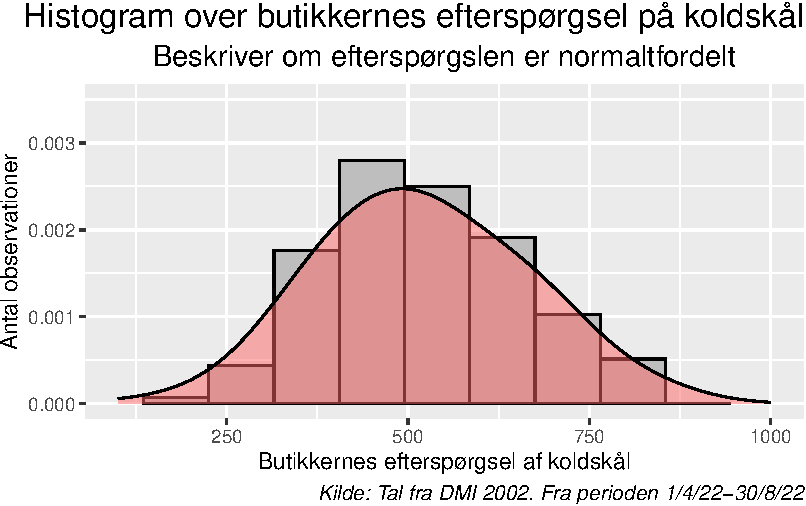
\includegraphics{Semester_projekt_2022_G1_files/figure-pdf/Chunk 7 - Histogram over efterspørgsel-1.pdf}

I følgende kode-chunk er der vist et boxplot. Det skal vise den
statistiske variationen ift. butikkens forventede lagerbeholdning og
efterspørgslen på koldskål. Man kan se at median-efterspørgslen stiger
fra høj til lav forventet lagerbeholdning af koldskål. Det tyder på at
der er en signifikant sammenhæng mellem de 2 variabler.

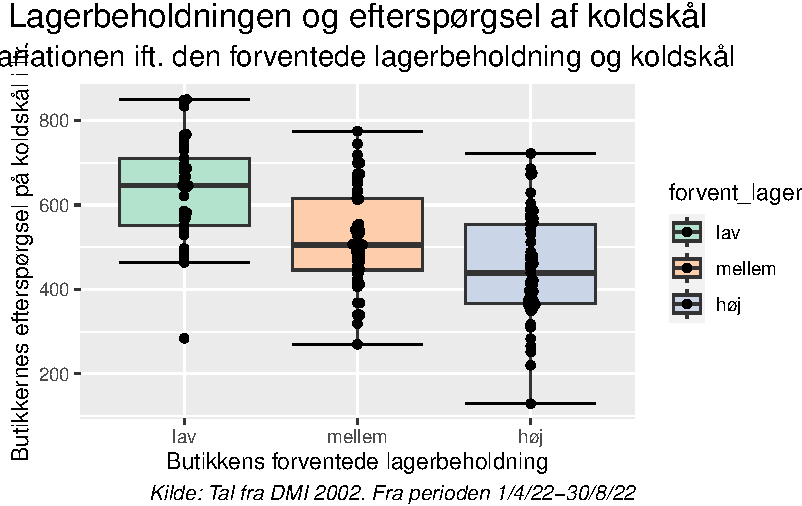
\includegraphics{Semester_projekt_2022_G1_files/figure-pdf/Chunk 8 - Boxplot over lagerbeholdning og efterspørgsel-1.pdf}

I næste kode-chunk er der lavet et boxplot som viser fordelingen af
efterspørgslen i forhold til om 25\% af butikkerne er løbet tør for
kammerjunkere eller ej. Hvis butikken har kammerjunkere på lager, er
efterspørgslen på koldskål højere, end hvis de ikke har kammerjunkere på
lager.

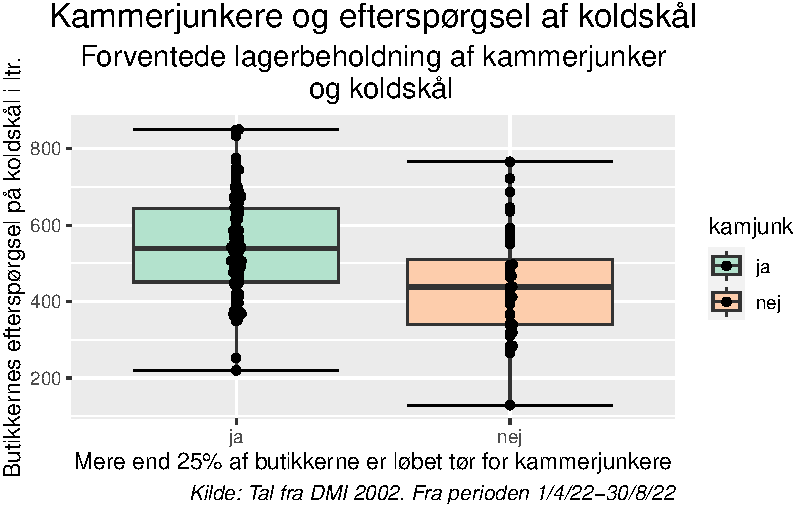
\includegraphics{Semester_projekt_2022_G1_files/figure-pdf/Chunk 9 - Boxplot over efterspørgsel og kammerjunkere-1.pdf}

Herunder er et boxplot som viser sammenhængen mellem måned og
efterspørgslen af koldskål. Det er tydeligt at se at
median-efterspørgslen stiger fra april-juli hvorefter efterspørgslen
igen falder i august.

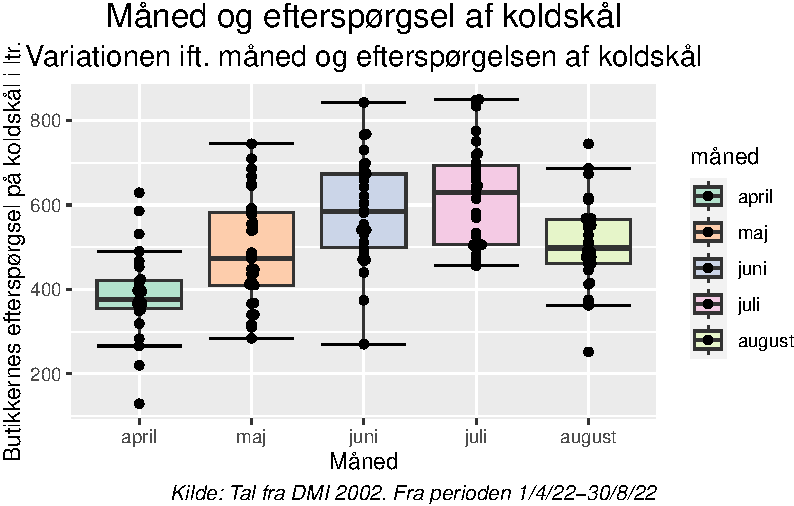
\includegraphics{Semester_projekt_2022_G1_files/figure-pdf/Chunk 10 - Boxplot over efterspørgsel og måned-1.pdf}

I nedestående kodechunk er der udvalgt 6 kontinuerte vejr-variabler, da
ønsket er, at undersøge om disse er korreleret med hinanden, og om deres
indbyrdes korrelation er statistisk signifikant. Der anvendes en
\texttt{chart.Correlation()} til at foretage en korrelationsanalyse.

Efterspørgel og humidity er ikke korreleret, og dermed ikke statistisk
signifikant. Beslutningen er derfor, at humidity ikke vil blive
inkluderet i analysen. Efterspørgsel og den gennemsnitlige temperatur
per time har en moderat korrelations koefficient på 0.38. P-værdien er
lav med tre stjerner, det betyder at sammenhængen er signifikant. Det er
derfor usandsynligt at opnå et mere ekstremt resultat, hvis man foretog
en ny undersøgelse. Mindre end \(5\%\) af korrelationen skyldes derfor
tilfældighed. Alle temperatur-variablerne er tæt på 1, hvilket betyder
at de har stærk samvariation. Dette kaldes for multikolinearitet. Det
vil sige, hvis de blev brugt i den endelige model ville det være
vanskeligt, at fortolke på koefficienterne. En Model med høj
multikolinearitet bliver mindre præcis og mindre pålidelig. For at
reducere multikolineariteten fjernes de øvrige temperatur-variable.

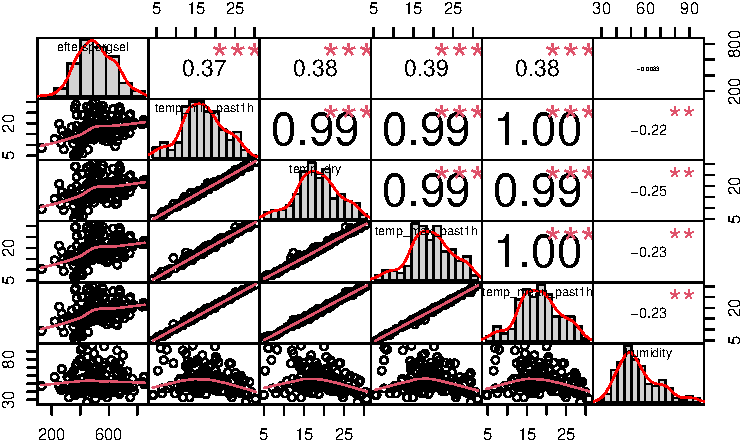
\includegraphics{Semester_projekt_2022_G1_files/figure-pdf/Chunk 11 - Korrelationsmatrice-1.pdf}

Som førnævnt var der en moderat signifikant sammenhæng mellem
efterspørgslen og gennemsnits temperaturen. Derfor bruges
temp\_mean\_past1h som den uafhængige effekt i næste kodechunk. Først
anvendes \texttt{predict()} til at konstruere et 95\(%
\) prædiktionsinterval, efterfulgt af \texttt{geom\_smooth()} til og
visualisere sammenhængen med et scatterplot.

Ud fra scatterplottet kan man se, at forholdet mellem den gennemsnitlige
temperatur og butikkernes efterspørgsel på koldskål er moderat lineært,
fordi hældningen på tendenslinjen er positiv. Det antages at når
gennemsnits temperaturen stiger én enhed, vil efterspørgslen stige
tilsvarende, det er `forholdsvis' mange af datapunkterne som er placeret
omkring tendenslinjen. Der anvendes lineær regression, fordi det er en
simpel metode, og det er nemt at tolke på model-parametrene. Mange af
datapunkterne ligger også langt væk fra tendenslinjen, der udtrykker en
stigende gennemsnitlig efterspørgsel på koldskål i ltr. Det indikerer at
der er stor varians og potentiel bias tilstede. En mere kompleks model
kan evt. anvendes til, at forklare sammenhængen yderligere. Flere af
observationerne er placeret udenfor dette bånd, hvorfor det er besluttet
at anvende et prædiktionsinterval i stedet - der er den røde stiplede
linje. Formålet er med andre ord, at medregne usikkerheden omkring de
individuelle værdier og ikke usikkerheden omkring gennemsnittet. Når den
gennemsnitlige temperatur hver time er 30 °C, er efterspørgslen på
koldskål for én ny observation 629.87 ltr. Ved samme temperatur vil
butikkernes efterspørgslen af koldskål med 95\% sikkerhed være
{[}369.30:890.43{]}. Man kan på baggrund af nedestående figur tydeligt
se, at hvis den gennemsnitlige temperatur i °C stiger, stiger
butikkernes efterspørgsel på koldskål tilsvarende.

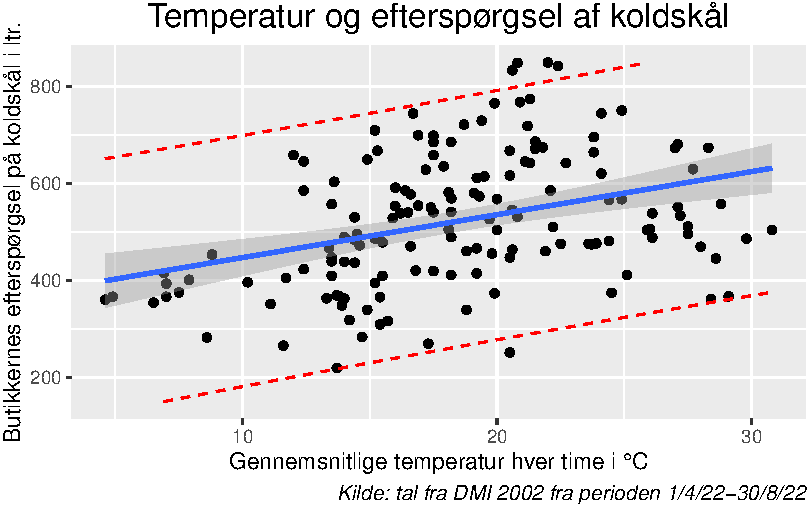
\includegraphics{Semester_projekt_2022_G1_files/figure-pdf/Chunk 12 - Scatterplot af temperatur og efterspørgsel-1.pdf}

\hypertarget{truxe6ning-puxe5-truxe6ningsdata}{%
\subsection{Træning på
træningsdata}\label{truxe6ning-puxe5-truxe6ningsdata}}

Først trænes modellen på træningsdata, fordi vi gerne vil tilpasse
modelparametrene. Der anvendes træningsdata til, at fintune vores
regressionsmodel. Efter modellen er trænet godt igennem, afprøves den på
testdata, da man gerne vil undersøge hvor god modellen er til, at
forudsige en så præcis efterspørgsel på koldskål som mulig. Vurderingen
af modelpræcisionen bestemmes ud fra den laveste MSE værdi. MSE måler
hvor langt den forudsagte værdi for en observation er fra den faktiske
værdi for en observation. Er MSE lille er der den forudsagte værdi tæt
på den faktiske værdi, er MSE stor er den forudsagte værdi langt fra den
faktiske værdi. MSE er således et udtryk for, hvor præcis den udvalgte
model er til, at forudsige efterspørgslen af koldskål (Hastie et.al
2021). MSE skal være så tæt på \(0\) som muligt.

Antallet af variabler i det samlede datasæt er mindre end antallet af
observationer. Derfor bruges backward-selection til, at udvælge de
uafhængige variabler som fremadrettet skal indgå i modellerne. Det vil
sige, at vi tilføjer alle variable ind på højre side af ligningen, og
fjerner dem med den højeste p-værdi. Indtil der kun er signifikante
uafhængige variable tilbage (Hastie et.al 2021). Denne teknik kan hjælpe
med at reducere unødvendig varians i den udvalgte model. men på samme
tid er den effektiv til, at identificere vigtige relationer i datasættet
(ibid).

\hypertarget{test-puxe5-testdata}{%
\subsection{Test på testdata}\label{test-puxe5-testdata}}

I det foregående afsnit blev den gennemsnitlige MSE beregnet for hver af
de fire modeller på træningsdata. Vi anvender ikke MSE for træningsdata.
Fordi det er mere interessant, at se hvor præcise forudsigelserne er på
testdata. Træningsdata anvendes som førnævnt til, at udvælge
signifikante uafhængige variable og tilpasse modelparametrene.

Dog er det værd at nævne, at den data undersøgelsen er baseret på
simulerede data. Dvs. at \(f\) er kendt allerede. Den virkelige sandhed
om efterspørgslen af koldskål vides dog ikke. Men hvis der bliver
udtrukket nogle testdata ud fra data3, kan man validere hvor godt en
model performer på disse testdata, når modelkompleksiteten øges.
Kompleksiteten kan øges ved, at de kontinuerte variable opløftes i flere
potenser, eller ved og inkludere flere uafhængige variabler som fx.
faktorer.

\hypertarget{metode-til-test-af-model-performance}{%
\subsection{Metode til test af model
performance}\label{metode-til-test-af-model-performance}}

Man kan producere testdata på flere måder. Der anvendes en \emph{LOOCV}
metode, fordi data3 kun indeholder 151 observationer i alt. Fordelen ved
fremgangsmåden er, at den træner på alle observationerne, undtagen ét
datapunkt. Processen gentages i dette tilfælde 150 gange. Derefter
beregnes en gennemsnitlig MSE score, som udtrykker hvor god
modelpræcisionen er (Hastie et.al 2021). Problemet med metoden er, at
det kræver stor computerkraft, det er fordi modellen trænes k gange
(ibid).

\begin{Shaded}
\begin{Highlighting}[numbers=left,,]
\NormalTok{ctrl }\OtherTok{\textless{}{-}} \FunctionTok{trainControl}\NormalTok{(}\AttributeTok{method =} \StringTok{"LOOCV"}\NormalTok{) }\CommentTok{\# Udvælger cross{-}validation metode}

\CommentTok{\# Baseline model}

\NormalTok{model0\_test }\OtherTok{\textless{}{-}} \FunctionTok{glm}\NormalTok{(efterspørgsel }\SpecialCharTok{\textasciitilde{}} \DecValTok{1}\NormalTok{ , }\AttributeTok{data =}\NormalTok{ data3)}
\NormalTok{cv.err1 }\OtherTok{\textless{}{-}} \FunctionTok{cv.glm}\NormalTok{(data3, model0\_test)}
\CommentTok{\#cv.err1$delta[[1]]}
\FunctionTok{rmse}\NormalTok{(model0\_test, }\AttributeTok{data =}\NormalTok{ data3) }\CommentTok{\# 139.1997}
\end{Highlighting}
\end{Shaded}

\begin{verbatim}
[1] 139.1997
\end{verbatim}

\begin{Shaded}
\begin{Highlighting}[numbers=left,,]
\CommentTok{\#model0\_test \# Gennemsnutlige efterspørgsel er 520.20 liter }

\CommentTok{\# Simpel model}

\NormalTok{model1\_test }\OtherTok{\textless{}{-}} \FunctionTok{train}\NormalTok{(efterspørgsel }\SpecialCharTok{\textasciitilde{}}\NormalTok{ temp\_mean\_past1h, }\AttributeTok{data =}\NormalTok{ data3, }
                     \AttributeTok{method =} \StringTok{"lm"}\NormalTok{, }\AttributeTok{trControl =}\NormalTok{ ctrl)}
\NormalTok{model1\_test }\CommentTok{\# RMSE 130.36}
\end{Highlighting}
\end{Shaded}

\begin{verbatim}
Linear Regression 

151 samples
  1 predictor

No pre-processing
Resampling: Leave-One-Out Cross-Validation 
Summary of sample sizes: 150, 150, 150, 150, 150, 150, ... 
Resampling results:

  RMSE      Rsquared   MAE     
  130.3607  0.1238588  105.8906

Tuning parameter 'intercept' was held constant at a value of TRUE
\end{verbatim}

\begin{Shaded}
\begin{Highlighting}[numbers=left,,]
\CommentTok{\#model1\_test \textless{}{-} summary(model1\_test)}
\CommentTok{\#model1\_test \# Printer alle modelparametre.}

\CommentTok{\# Moderat model}

\NormalTok{model2\_test }\OtherTok{\textless{}{-}} \FunctionTok{train}\NormalTok{(efterspørgsel }\SpecialCharTok{\textasciitilde{}}\NormalTok{ forvent\_lager }\SpecialCharTok{+}
\NormalTok{                       weekend\_helligdag }\SpecialCharTok{+}\NormalTok{ måned }\SpecialCharTok{+}
\NormalTok{                       kamjunk }\SpecialCharTok{+} 
\NormalTok{                       temp\_gt25\_3\_dage }\SpecialCharTok{+} 
                       \FunctionTok{I}\NormalTok{(temp\_mean\_past1h}\SpecialCharTok{\^{}}\DecValTok{1}\NormalTok{), }\AttributeTok{data =}\NormalTok{ data3,}
                       \AttributeTok{method =} \StringTok{"lm"}\NormalTok{, }\AttributeTok{trControl =}\NormalTok{ ctrl)}
\CommentTok{\#model2\_test \# RMSE 88.55}
\CommentTok{\#model2\_test \textless{}{-} summary(model2\_test)}
\NormalTok{model2\_test }\CommentTok{\# Printer alle modelparametre.}
\end{Highlighting}
\end{Shaded}

\begin{verbatim}
Linear Regression 

151 samples
  6 predictor

No pre-processing
Resampling: Leave-One-Out Cross-Validation 
Summary of sample sizes: 150, 150, 150, 150, 150, 150, ... 
Resampling results:

  RMSE      Rsquared   MAE     
  88.55084  0.5967607  72.56083

Tuning parameter 'intercept' was held constant at a value of TRUE
\end{verbatim}

\begin{Shaded}
\begin{Highlighting}[numbers=left,,]
\CommentTok{\# Kompleks model}

\NormalTok{model3\_test }\OtherTok{\textless{}{-}} \FunctionTok{train}\NormalTok{(efterspørgsel }\SpecialCharTok{\textasciitilde{}}\NormalTok{ forvent\_lager }\SpecialCharTok{+} 
\NormalTok{                       weekend\_helligdag }\SpecialCharTok{+}
\NormalTok{                       kamjunk }\SpecialCharTok{+} 
\NormalTok{                       temp\_gt25\_3\_dage }\SpecialCharTok{+} 
\NormalTok{                       måned }\SpecialCharTok{+}
                       \FunctionTok{I}\NormalTok{(temp\_mean\_past1h}\SpecialCharTok{\^{}}\DecValTok{22}\NormalTok{), }\AttributeTok{data =}\NormalTok{ data3, }
                       \AttributeTok{method =} \StringTok{"lm"}\NormalTok{, }\AttributeTok{trControl =}\NormalTok{ ctrl)}
\NormalTok{model3\_test }\CommentTok{\# RMSE 89.37393}
\end{Highlighting}
\end{Shaded}

\begin{verbatim}
Linear Regression 

151 samples
  6 predictor

No pre-processing
Resampling: Leave-One-Out Cross-Validation 
Summary of sample sizes: 150, 150, 150, 150, 150, 150, ... 
Resampling results:

  RMSE      Rsquared   MAE     
  89.37393  0.5890984  72.52832

Tuning parameter 'intercept' was held constant at a value of TRUE
\end{verbatim}

\begin{Shaded}
\begin{Highlighting}[numbers=left,,]
\CommentTok{\#model3\_test \textless{}{-} summary(model3\_test)}
\NormalTok{model3\_test }\CommentTok{\# Printer alle modelparametre.}
\end{Highlighting}
\end{Shaded}

\begin{verbatim}
Linear Regression 

151 samples
  6 predictor

No pre-processing
Resampling: Leave-One-Out Cross-Validation 
Summary of sample sizes: 150, 150, 150, 150, 150, 150, ... 
Resampling results:

  RMSE      Rsquared   MAE     
  89.37393  0.5890984  72.52832

Tuning parameter 'intercept' was held constant at a value of TRUE
\end{verbatim}

\hypertarget{resultater}{%
\section{Resultater}\label{resultater}}

Nu er de fire modeller blevet trænet på træningsdata og testet godt
igennem på testdata. Resultaterne tager kun udgangspunkt i
koefficienterne fra de fire testmodeller. Modellen med den laveste
kvadrerede RMSE, og den højeste \(R^2\) er den model som har størst
præcision.

Baselinemodellen har kun den afhængige variabel i ligningen.
\(\hat{\beta_0}\) er den gennemsnitlige efterspørgsel på koldskål ved
\(520.23\) ltr. \(RMSEtest=139.20\). Bliver Temp\_mean\_past1h
inkluderet i den simple model, falder \(RMSEtest=130.36\), det betyder
at modellen `fitter' bedre på data og at modellen har højere præcision.
Inkluderes de kategoriske faktorer i modellen med moderat kompleksitet,
falder \(RMSEtest=88.55\) . Det er den model hvor den forudsagte værdi
er tættest på den faktiske værdi. Dertil er \(adjR^2 = 0.63\%\), det
referer til den proportion af butikkernes efterspurgte koldskål som
bliver forklaret af de uafhængige variabler. De forklarer altså 63\% af
den samlede varians i datasættet.

Bliver modellen mere kompleks, bliver præcisionen ikke altid bedre -
ofte gælder det modsatte! I den komplekse model stiger
\(RMSEtest=89.37\) og \(adjR^2 = 0.62\%\) falder. Desuden bliver
Temp\_mean\_past1h\^{}22 insignifikant, da hældningen er 0. Det skyldes
muligvis overfitting.

Den moderate model er blevet udvalg til den mest præcise model, fordi
den har lavest RMSE. Fortolkningen af koefficienterne er, når de øvrige
variabler holdes konstant:

\begin{itemize}
\item
  Er den forventede lagerbeholdning på mellemste niveau, falder
  butikkernes gennemsnitlige efterspørgsel på koldskål med \(-76.57\)
  ltr, i forhold til butikker med en lav forventet lagerbeholdningen.
\item
  Er den forventede lagerbeholdning på højeste niveau, falder
  butikkernes gennemsnitlige efterspørgsel på koldskål med \(-82.67\)
  ltr, i forhold til butikker med en lav forventet lagerbeholdning.
  Ændres referencegruppen, stiger efterspørgslen tilsvarende.
\end{itemize}

Det giver umiddelbart god mening, da butikkerne ikke vil risikere at
bestille for meget koldskål. Da der er risiko for, at den ikke bliver
solgt, og dermed øges riskoen for, at koldskålen overskrider sidste
salgsdato.

\begin{itemize}
\tightlist
\item
  Er 25\% af butikkerne i det pågældende område ikke løbet tør for
  kammerjunkere, falder butikkernes gennemsnitlige efterspørgsel med
  \(-71.89\) ltr, sammenlignet med de 25\% af butikkerne i det
  pågældende som er løbet tør for kammerjunkere. Ændres
  referencegruppen, stiger efterspørgslen tilsvarende.
\end{itemize}

Butikkerne vil gerne lave mersalg og dermed sælge kammerjunkere sammen
med koldskål. Det kan også indikere at forbrugerne synes koldskål og
kammerjunkere skal spises sammen.

\begin{itemize}
\tightlist
\item
  I maj måned stiger butikkernes efterspørgsel på koldskål
  gennemsnitligt med \(84.37\) ltr, i forhold til april måned. I juni
  måned stiger efterspørgslen gennemsnitligt med \(129.51\) ltr, i
  forhold til april måned. I juli måned stiger efterspørgslen
  gennemsnitligt med \(155.95\) ltr, i forhold til april måned. I august
  falder efterspørgslen ned til \(85.10\) ltr, sammenlignet med april
  måned.
\end{itemize}

Det betyder, at butikkernes gennemsnitlige efterspørgsel på koldskål
stiger hen over sommeren til og med august, hvor sæsonen nærmer sig
slutningen (Holland 2022)

\begin{itemize}
\tightlist
\item
  Har der været 25°C eller varmere i mere end tre dage, falder
  butikkernes gennemsnitlige efterspørgsel på koldskål med \(-66.74\)
  ltr.
\end{itemize}

Det kan være en indikation på, at forbrugerne bliver trætte af at spise
koldskål, når det bliver for varmt over en længere periode.

\begin{itemize}
\tightlist
\item
  Stiger den gennemsnitlige temperatur målt pr. time med én °C, stiger
  butikkernes efterspørgsel på koldskål i gennemsnit med \(4.25\) ltr.
\end{itemize}

Øget sommervarme hænger moderat sammen med butikkernes efterspørgsel på
koldskål. Det stemmer overens med eksisterende viden på området (Kjer
2022).

\begin{longtable}[]{@{}
  >{\raggedright\arraybackslash}p{(\columnwidth - 8\tabcolsep) * \real{0.2990}}
  >{\centering\arraybackslash}p{(\columnwidth - 8\tabcolsep) * \real{0.1649}}
  >{\centering\arraybackslash}p{(\columnwidth - 8\tabcolsep) * \real{0.1649}}
  >{\centering\arraybackslash}p{(\columnwidth - 8\tabcolsep) * \real{0.1649}}
  >{\centering\arraybackslash}p{(\columnwidth - 8\tabcolsep) * \real{0.1753}}@{}}
\toprule()
\begin{minipage}[b]{\linewidth}\raggedright
\end{minipage} & \begin{minipage}[b]{\linewidth}\centering
\textbf{Baseline}
\end{minipage} & \begin{minipage}[b]{\linewidth}\centering
\textbf{Simpel}
\end{minipage} & \begin{minipage}[b]{\linewidth}\centering
\textbf{Moderat}
\end{minipage} & \begin{minipage}[b]{\linewidth}\centering
\textbf{Kompleks}
\end{minipage} \\
\midrule()
\endhead
\textbf{Forvent\_lager (mellem)} & & & \(-76.57\)\(***\)

\{\(19.82\)\} & \(-74.55\)\(***\)

\{\(19.72\)\} \\
\textbf{Forvent\_lager (høj)} & & & \(-82.67\)\(***\)

\{\(22.58\)\} & \(-87.00\)\(***\)

\{\(22.81\)\} \\
\textbf{Weekend\_helligdag (ja)} & & & \(113.01\)\(***\)

\{\(15.00\)\} & \(107.33\)\(***\)

\{\(15.16\)\} \\
\textbf{Kamjunk (nej)} & & & \(-71.89\)\(***\)

\{\(17.50\)\} & \(-76.52\)\(***\)

\{\(19.82\)\} \\
\textbf{Temp\_gt25\_3\_dage} & & & \(-82.00\)\(*\)

\{\(34.23\)\} & \(-66.74\)\(*\)

\{\(34.90\)\} \\
\textbf{Måned (maj)} & & & \(84.37\)\(***\)

\{\(24.54\)\} & \(101.69\)\(***\)

\{\(23.36\)\} \\
\textbf{Måned (juni)} & & & \(129.51\)\(***\)

\{\(32.79\)\} & \(162.71\)\(***\)

\{\(27.87\)\} \\
\textbf{Måned (juli)} & & & \(155.95\)\(***\)

\{\(32.79\)\} & \(155.947\)\(***\)

\{\(29.12\)\} \\
\textbf{Måned (august)} & & & \(85.10\)\(*\)

\{\(34.76\)\} & \(197.44\)\(*\)

\{\(30.96\)\} \\
\textbf{Temp\_mean\_past1h} & & \(9.46\)\(***\)

\{\(1.89\)\} & \(4.249\)\(*\)

\{\(2.07\)\} & \(0\) \\
Uafhængige variable & \(0\) & \(1\) & \(6\) & \(6\) \\
Skæring \(\hat{\beta_0}\) & \(520.23\)\(***\) & \(346.04\)\(***\) &
\(379.93\)\(***\) & \(434.78\)\(***\) \\
Model P-værdi & \(***\) & \(***\) & \(***\) & \(***\) \\
RMSE\_træning & \(139.20\) & \(128.74\) & \(82.10\) & \(83.21\) \\
RMSE\_test & \(139.20\) & \(130.36\) & \(88.55\) & \(89.37\) \\
\(R^2\) & & \(0.15\%\) & \(0.65\%\) & \(0.64\%\) \\
Justeret \(R^2\) & & \(0.14\%\) & \(0.63\%\) & \(0.62\%\) \\
Observationer & \(151\) & \(151\) & \(151\) & \(151\) \\
\bottomrule()
\end{longtable}

Tabel 1. Summeret modelreferat fra testdata. Referencegrupper () for
faktorerne er: kamjunkja, forvent\_lagerlav, månedapril. \{\} referer
til standardfejlen. Note:\(* = P < 0.1; ** = P < 0.05; *** = P <0.01\)

\hypertarget{diskussion}{%
\section{Diskussion}\label{diskussion}}

Først laves der et histogram med \texttt{ggplot()} der viser forskellen
i RMSE for alle modellerne på hhv. test og træningsdata ud fra
modelkomplesiteten. Forskellen i trænings- og test RMSE er jvf.
histogrammet ikke ens når kompleksiteten øges. Det samme mønster i den
moderate og den komplekse gælder. Det er en generel tendens, at test
RMSE er større end træningsRMSE, når modelkompleksiteten stiger.

Det skyldes at LOOCV-metoden `tuner' modellerne for meget, så den køre
modellen for hårdt på træningsdata. På den måde opfanger modellen
tilfældigheder fra træningsdata, i stedet for egenskaber ved den \(f\),
vi ikke kender til. Mønstret fra træningsdata stemmer dermed ikke
overens med mønstret i testdatasættet (Hastie 2022). I dette tilfælde er
testRMSE højere på testdata end på træningsdata kaldes det for
overfitting. I histogrammet kan man også se, at forskellen mellem RMSE i
den moderate og den komplekse model er meget lille. Alt andet lige,
vælges den moderate ud fra et princip om sparsommelighed frem for den
komplekse model (ibid).

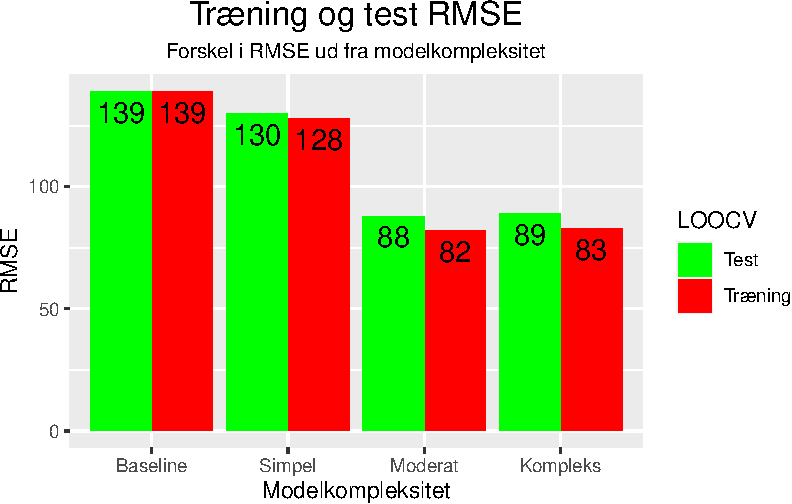
\includegraphics{Semester_projekt_2022_G1_files/figure-pdf/Chunk 15 - Histgram over MSE-1.pdf}

For det første hænger det optimale metodevalg sammen med præcision i
forudsigelse og fortolkningen af parametrene. Stiger fleksibiliteten
bliver det svære at tolke på parametrene. Falder falder fleksibiliteten
bliver det nemmere at tolke på parametrene. Da Temp\_mean\_past1h blev
opløftet til Temp\_mean\_past1h\^{}22 i den komplekse model, blev p
værdien for \(\hat{\beta_1}\) for insignifikant ved \(Pr = 0.58\%\).
\(\hat{\beta_1}\) er derfor ikke tilstrækkelig langt fra \(0\). Dette
gjorde det vanskeligere at tolke på denne paramter. Det er fordi
modellen opfangede for mange fejl og for meget støj i form af varians.

For det andet hænger modelvalget sammen det bias/variance tradeoff som
forekommer, hvis man øger modelkompleksiteten i jagten på identificere
den model som har lavest varians og bias. Varians er ændringen i
\(\hat{f}\), når den beregnes på nye data - men værdien er aldrig helt
den samme! Stiger fleksibiliteten øges variansen. Bias opstår når man
forsøger, at forudsige et komplekst fænomen med en for simpel metode.
Stiger fleksibiliteten reduceres bias (ibid). Efterspørgslen på koldskål
er som førnævnt et multidimensionelt fænomen. Vi forsøgte at reducere
bias ved og udvide den simple lineære model med Temp\_mean\_past1h uden
alle de kategoriske faktorvariabler, da de ikke kan indgå i en
polynomisk regression (ibid). Det resulterede ikke i en forbedring i
RMSE, eller en stigning i \(R^2\). Hverken da den blev opløftet i 3 og
22 potens. Valget blev derfor, at beholde faktorerne i den moderate
model, fordi de til sammen forklarer \(63\%\) af variansen. Andre
variable kunne havde indflydelse på butikkernes efterspørgsel på
koldskål. Gennemsnitlige antal solskinstimer, maksimale vindhastighed,
samt de private forbrugers socioøkonomiske forhold kunne bidrage med
flere dimensioner til den moderate model. Beslutningen blev derfor, at
vælge den multible lineære model med moderat kompleksitet. I næste
kapitel udrulles anbefalingerne.

\hypertarget{anbefalinger}{%
\section{Anbefalinger}\label{anbefalinger}}

For at kunne designe og udvikle det bedste dataprodukt bruges et Data
Product Canvas til, at kortlægge nøgleområder i form af anbefalinger.
Thise skal implementere disse for, at øge deres datamodenhed og dermed
øge deres økonomiske indtjeningspotentiale. Der præsenteres fem
overordnede anbefalinger:

\begin{enumerate}
\def\labelenumi{\arabic{enumi}.}
\item
  Opgradér Navision til også at være sky-baseret, i stedet for
  udelukkende at bruge det via. Windows styresystemet.
\item
  Brug den multible lineære regression fra analysen som modelskabelon,
  og reproducer den i en anden produktionskontekst. Modellen er:
  \(\hat{efterspørgsel} = \hat{forventlager} + \hat{kamjunk} + \hat{maaned} + \hat{tempmeanpast1h} + \hat{tempgt3dage} + \hat{weekendhelligdag}\)
\item
  Medarbejderne skal opfattes sig selv som værende en del af en moderne
  datamodenhedskultur. Første skridt er at ansatte en dataanalytiker som
  skal accelerer datamodenhedsprocessen fra fase til fase to. I fase to
  begynder man at strukturere dataopsamlingen for, at lukke risikohuller
  der er når forskellige systemer skal samarbejde.
\item
  Ledelsen skal være spydspidsen når datamodenhedsprocessen skal
  acceleres fremadrettet.
\item
  Brug R-Studio som programmeringssprog fordi det er gratis og det
  arbejder godt sammen med andre programmer som fx. SQL.
\end{enumerate}

\hypertarget{konklusion}{%
\section{Konklusion}\label{konklusion}}

Thise Mejeri er på fase 1 i Alexandramodellen, hvor de i stor grad
bruger deres data til, at spore driften af produktionsafdelingen. De kan
forbedre deres datamodenhed ved, at arbejde mere struktureret med
dataopsamlingen og anvendelse heraf.

For at styrke den fremtidige leveringsscore hos COOP, skal Thise Mejeri
reproducere den multiple lineære regressionsmodel i flere
produktionssammenhænge fremadrettet, holdt op i mod vejrdata fra DMI.

\hypertarget{litteratur}{%
\section{Litteratur}\label{litteratur}}

Bækby, R. \& Kølsen, C. (marts. 2017). \emph{„Find din vej i
dataindsatsen''}. I: Alexandrainstituttet.

Hastie, T. \& James, G. (august. 2021). \emph{„An introduction to
statistical learning''}. I: Springer. 2 udgave.

Holland, S. (jul. 2022). \emph{„Vejret afgør sommerens mængde af
koldskål''}. I: Fødevareforbundet.

\textbf{Link:}
\url{https://www.nnf.dk/nyheder/2021/juli/vejret-afgor-sommerens-maengde-af-koldskal}

Jensen, M. L (jul. 2022). \emph{„Thise skruer gevaldigt op for
koldskålsproduktionen''}. I: Tv Midtvest.

\textbf{Link:}
\url{https://www.tvmidtvest.dk/skive/thise-mejeri-skruer-gevaldigt-op-for-koldskaalsproduktionen}

Kjer, U. (sep. 2022). „\emph{Sommervejret var 3 pct. bedre end sidste
år''}. I: Mejeriforeningen.

\textbf{Link:}
\url{https://mejeri.dk/nyheder/sommervejret-var-3-pct-bedre-end-sidste-ar/}

Osterwalder, A. \& Pigneur, Y. (2010). \emph{„Business Model Generation
``}. 1. udgave. John Wiley \& Sons.

Picopublish (feb. 2022). \emph{„Datamodenhed handler om at blive bedre
til at anvende egne data i værdiskabende sammenhænge''}. I: Picopublish.

Jensen, S. (nov, 2022), \emph{„Interview med Søren Jensen på Thise
Mejeri''.} Kenneth, Eva og Sanne.

\hypertarget{sessioninformation}{%
\section{Sessioninformation}\label{sessioninformation}}

\begin{Shaded}
\begin{Highlighting}[numbers=left,,]
\FunctionTok{sessionInfo}\NormalTok{(}\AttributeTok{package =} \ConstantTok{NULL}\NormalTok{) }\CommentTok{\# Printer en liste om R sessionen.}
\end{Highlighting}
\end{Shaded}

\begin{verbatim}
R version 4.2.1 (2022-06-23)
Platform: x86_64-apple-darwin17.0 (64-bit)
Running under: macOS Big Sur ... 10.16

Matrix products: default
BLAS:   /Library/Frameworks/R.framework/Versions/4.2/Resources/lib/libRblas.0.dylib
LAPACK: /Library/Frameworks/R.framework/Versions/4.2/Resources/lib/libRlapack.dylib

locale:
[1] en_US.UTF-8/en_US.UTF-8/en_US.UTF-8/C/en_US.UTF-8/en_US.UTF-8

attached base packages:
[1] splines   stats     graphics  grDevices utils     datasets  methods  
[8] base     

other attached packages:
 [1] kableExtra_1.3.4           stargazer_5.2.3           
 [3] pscl_1.5.5                 car_3.1-0                 
 [5] carData_3.0-5              PerformanceAnalytics_2.0.4
 [7] xts_0.12.2                 zoo_1.8-11                
 [9] writexl_1.4.1              openxlsx_4.2.5            
[11] boot_1.3-28.1              RColorBrewer_1.1-3        
[13] palmerpenguins_0.1.1       ggbeeswarm_0.6.0          
[15] tinytex_0.43               timeDate_4021.104         
[17] readxl_1.4.1               viridis_0.6.2             
[19] viridisLite_0.4.0          fueleconomy_1.0.0         
[21] nasaweather_0.1            babynames_1.0.1           
[23] class_7.3-20               RSQLite_2.2.16            
[25] caret_6.0-93               lattice_0.20-45           
[27] leaps_3.1                  testthat_3.1.5            
[29] MASS_7.3-58.1              ISLR2_1.3-1               
[31] microbenchmark_1.4.9       jsonlite_1.8.0            
[33] httr_1.4.4                 XML_3.99-0.10             
[35] modelr_0.1.9               pander_0.6.5              
[37] broom_1.0.1                htmlwidgets_1.5.4         
[39] feather_0.3.5              hexbin_1.28.2             
[41] hms_1.1.2                  pryr_0.1.5                
[43] lubridate_1.8.0            maps_3.4.1                
[45] Lahman_10.0-1              gapminder_0.3.0           
[47] nycflights13_1.0.2         magrittr_2.0.3            
[49] forcats_0.5.2              stringr_1.4.1             
[51] dplyr_1.0.10               purrr_0.3.4               
[53] readr_2.1.2                tidyr_1.2.0               
[55] tibble_3.1.8               ggplot2_3.4.0             
[57] tidyverse_1.3.2           

loaded via a namespace (and not attached):
 [1] backports_1.4.1      systemfonts_1.0.4    plyr_1.8.7          
 [4] listenv_0.8.0        digest_0.6.29        foreach_1.5.2       
 [7] htmltools_0.5.3      fansi_1.0.3          memoise_2.0.1       
[10] googlesheets4_1.0.1  tzdb_0.3.0           recipes_1.0.1       
[13] globals_0.16.1       gower_1.0.0          svglite_2.1.0       
[16] hardhat_1.2.0        colorspace_2.0-3     blob_1.2.3          
[19] rvest_1.0.3          haven_2.5.0          xfun_0.32           
[22] crayon_1.5.1         survival_3.3-1       iterators_1.0.14    
[25] glue_1.6.2           gtable_0.3.0         gargle_1.2.0        
[28] ipred_0.9-13         webshot_0.5.3        future.apply_1.9.1  
[31] abind_1.4-5          scales_1.2.1         DBI_1.1.3           
[34] Rcpp_1.0.9           bit_4.0.4            stats4_4.2.1        
[37] lava_1.6.10          prodlim_2019.11.13   ellipsis_0.3.2      
[40] farver_2.1.1         pkgconfig_2.0.3      nnet_7.3-17         
[43] dbplyr_2.2.1         utf8_1.2.2           labeling_0.4.2      
[46] tidyselect_1.1.2     rlang_1.0.6          reshape2_1.4.4      
[49] munsell_0.5.0        cellranger_1.1.0     tools_4.2.1         
[52] cachem_1.0.6         cli_3.4.1            generics_0.1.3      
[55] pacman_0.5.1         evaluate_0.16        fastmap_1.1.0       
[58] yaml_2.3.5           ModelMetrics_1.2.2.2 knitr_1.40          
[61] bit64_4.0.5          fs_1.5.2             zip_2.2.0           
[64] future_1.28.0        nlme_3.1-157         xml2_1.3.3          
[67] brio_1.1.3           compiler_4.2.1       rstudioapi_0.13     
[70] curl_4.3.2           beeswarm_0.4.0       reprex_2.0.2        
[73] stringi_1.7.8        Matrix_1.4-1         vctrs_0.5.1         
[76] pillar_1.8.1         lifecycle_1.0.3      data.table_1.14.2   
[79] R6_2.5.1             gridExtra_2.3        vipor_0.4.5         
[82] parallelly_1.32.1    codetools_0.2-18     assertthat_0.2.1    
[85] withr_2.5.0          mgcv_1.8-40          parallel_4.2.1      
[88] quadprog_1.5-8       grid_4.2.1           rpart_4.1.16        
[91] rmarkdown_2.16       googledrive_2.0.0    pROC_1.18.0         
[94] ggeasy_0.1.3        
\end{verbatim}

\hypertarget{bilag}{%
\section{Bilag}\label{bilag}}

Bilag 1 - Interviewguide.

\includegraphics{images/Skærmbillede 2022-12-29 kl. 21.17.40.png}

\includegraphics{images/Skærmbillede 2022-12-29 kl. 21.19.03.png}

\includegraphics{images/Skærmbillede 2022-12-29 kl. 21.19.47.png}

\includegraphics{images/Skærmbillede 2022-12-29 kl. 21.20.28.png}

\includegraphics{images/Skærmbillede 2022-12-29 kl. 21.21.00.png}

\includegraphics{images/Skærmbillede 2022-12-29 kl. 21.21.31.png}

Bilag 2~

Interview af Søren Jensen fra produktionsafdelingen i Thise Mejeri ~\\
Gruppe 1~

3. november 2022~

Søren fortæller at de producerer helst over midnat så de kan skrive den
nye dato på pakken. Han fortæller at de producerer ud fra en statistik
og hvis de skal forudsige produktionen af koldskål, så skal de være en
form for metrologer. De skal være ekstra opmærksomme på statistik fra
tidligere år da klimaforandring gør at sommeren har forandret sig.
Salget er ofte højest i starten af sommerperioden og Thise indsamler
data på dette.

Hver dag omkring middag kommer ordrerne fra Coop og produktionen håber
at det stemmer nogenlunde overens med det de har tappet. Hvis ikke skal
de lav en ekstra tapning ellers kan Coop godt godkende det til næste dag
hvis det er en lille procent. Der skal minimum være 8 terminaldage når
Coop får det leveret.~~

Koldskål er utrolig afhængig af vejret. Udefrakommende faktorer har også
en afgørende rolle; eks. Hvis Arla sælger koldskål til 5 kr. Thise har
mange loyale kunder og et godt image men store besparelser fra
konkurrenter kan være afgørende for salget hos Thise. Når Thise har et
nyt produkt de vil afprøve, så starter de i Irma og hvis det lykkedes,
så går det videre til Coop. Thise sælger kun helårs koldskål i Irma og i
uge 27-36 sælges det andre steder.~~

Koldskålproduktionen foregår ved at man tager kærnemælk over og syrner
det, så ryger det i en tank som snurrer rundt og der hældes fløde i og
kærnemælken tappes af og blandes med en frugtmix af vanilje og æg.~ Ca.
15\% mix og 85\% kærnemælk. Der kan produceres ca. 5-6 ton koldskål i
timen på 1 tap.~~

Kærnemælkdrengen (en erfaren mejerist) sørger for at ph-værdigen er lav
nok og produktionen smager også på produktet. Laboratoriet udvælger den
første og den sidste og 3 i midten til at smage på hver dag og giver
karakter på en 15-trins skala. På den måde kan de nå at stoppe salget
hvis det smager dårligt. Karakteren gives for ydre, konsistens, lugt og
smag. 15 er fantastisk.~

Ifølge Søren, så er medarbejdernes it-kompetencer i produktionen ikke
høj.~

Medarbejderne i Thise har typisk været ansat i firmaet i lang tid. Søren
har arbejdet hos Thise siden konfirmandsalderen.~

Bilag 3~

\begin{itemize}
\item
  Interview med salgschef Peter Pedersen hos Thise Mejeri~

  Gruppe 4~

  Interview information:~

  Informanten:~

  Peter Pedersen: salgchef Asien~

  \textbf{SP 1:}~

  Hvad underbygger i jeres markedsføring i Asien på?~

  Svar:~

  Der laves overhovedet ingen markedsføring i Asien. Det er B2B -- dvs
  ingen kontakt med slutkunder.~

  \textbf{SP2:}~

  Hvis I fik data, hvordan vil I markedsføre jer til det Kinesiske
  marked for eksempel?~

  Svar:~

  Det Kinesiske marked er meget forskelligt fra det Danske marked. Meget
  af marketing er trukket over på de sociale medier. Det er meget,
  tungere på ``influencer'' end i den vestlige verden. Kinesiske
  influencers tjener mange flere penge end vestlige influencers. Det er
  et helt andet marked man skal penetrere end, hvis man gerne vil til
  Tyskland. I Tyskland kan man reklamere i fagblade, f.eks. i
  økofagblade.~

  Hvis man skal slå sig igennem Asien så er det en rigtig god idé at få
  de her influencer igennem som er på forskellige platforme (f.eks.
  TikTok) og andre kinesisk sociale medie platforme som vi ikke kender
  til i Danmark. Det kræver også noget som en organisation at sætte sig
  ind i hvordan man egentlig får mest muligt ud af de platforme.~

  Thise har været i gang med det på et tidspunkt at oprette en online
  ``store'' på noget der hedder ``T-mall'' (?). Det kan sammenlignes med
  Amazon. De kan oprette en Thise butik på T-mall hvor de så kunne sælge
  oste igennem. Det kom de aldrig videre pga logistiske problemer ift
  distribution i Kina, fordi Kina er ret stor. Der er mange byer hvor
  der bor mindst 10 millioner mennesker. Hvor skal man distribuere ud
  fra hvis, man gerne vil ud til Tangchon (en by i Kina? Jeg ved ikke
  hvordan det staves) som, man byggede Jeg? Har været i med tolv
  millioner mennesker man, aldrig har hørt om før Er. Det nok og have
  distribution i Beijing hvor, der er to hundrede kilometer fra til
  Tanchan? Eller skal man også have en distribution i Tanchan. For en
  lille organisation som Thise er det meget svært. Den idé var derfor
  droppet det igen. Ellers skal man kunne have cold-chain distribution
  af mælk, smør og ost fra Thise til Kina -- noget der har store
  udfordringer. Det er svært og meget dyrt.~

  De har ikke et markedsføringsbudget. De laver produkter med gode
  historier. De almindelige media (f.eks. Folkeblad) tager historien op,
  og så laver de faktisk deres markedsførings for dem. Det er den måde
  de har drevet Thise Mejeri helt fra starten af. Det er, at de har
  lavet gode produkter med gode historier som, de ikke har puttet penge
  i at få det fortalt.~

  \textbf{SP3:}~

  Samles der information om hvordan reklamer/historier i Folkeblad har
  påvirket jeres salg af produkterne?~

  Svar:~

  Ikke helt ned på produktniveau. Der er nogen i
  kommunikationsafdelingen som holder styr på hvor meget omtale de får -
  om den er positiv eller negativ.~

  De havde en tilbagetrækning for et halvt års tid siden, fordi der var
  solgt nogle liter mælk med rengøringsvæske i. Der har ikke været styr
  på rengøringsprocessen. Der kunne de se at de historier der bliver
  skrevet rundt omkring var knap så positive som de plejer at være. De
  ``tracer'' alt efter om det er godt eller skidt omtale, og har som
  konsekvens af det fjernet soja og måler heraf aktiviteten i omtalen
  for ligeledes at kunne vurdere om der er stingende positiv eller
  negativ omtale. Tracer også trafik på sociale medier~

  \textbf{SP4:}~

  Hvordan deler I med coop denne salgsinformation, som resultat af jeres
  samarbejde?~

  Svar:~

  Det er jeg faktisk ikke klar over. Vi har en ret unik måde at
  samarbejde med dem på. Det er egentlig os, der sender varer til Coop
  før de sender en ordre til os. Vi forecaster på, hvor meget Coop skal
  have, og så sender vi det derover. Der bliver sendt varer tilsvarende
  forecasten om morgenen, hvor Coop så sender deres ordre i løbet af
  eftermiddagen. Estimeret 90\% af de varer Coop bestiller er allerede
  sendt, da Thise forecaster korrekt. Derfor bliver det de
  supplerende/manglende mængder, der leveres om aftenen. ~\\
  Forud for dette er der en række data, der er tilgængelig for Thiese
  fra Coop, blandt andet lagerbeholdning. Dog er informanten ikke klar
  over de konkrete metoder til at samle og modtage disse data.~~

  \textbf{SP5:}~

  Hvor opsamler I jeres salgsdata fra Coop?~

  Svar:~

  Vi har en afdeling, hvor de ansatte sidder med deres forecast -- med
  ca. 6-8 mand, der planlægger produktionen. På grund af den store
  mængde forskellige produkter, og derfor varenumre, så er det
  nødvendigt med en stor mængde data, hvilke er tilgængelige i
  føromtalte afdeling. Udover Coop (som er ca halvdelen af
  forretningen), så er der endnu flere datakilder.~

  \textbf{SP6:} ~

  Er Coop med til produktudvikling? Eller er der andre af jeres kunder,
  der har indvirkning på udvikling?~

  Svar:~

  Ja, de er en aktiv medspiller. Nogle gange har Coop en idé om et
  produkt de gerne vil have, det kan feks være et eksisterende produkt
  som de ønsker i en økologisk udgave, så kan de kontakte os for at høre
  om det er noget vi kan producere. De er en stærk medspiller, og de
  fleste produkter bliver født her i Thiese, og så banker vi på ved Coop
  for at høre om de er interesserede i at sælge dem -- hvilket de oftest
  gerne vil. I mange år har vi haft et meget tæt samarbejde med Irma,
  som vi har brugt en del til at teste markedet af, fordi Irma
  butikkerne lever af at have et nyt og spændende sortiment -- med stor
  udskiftning -- så når vi har et nyt produkt, så ringer vi mere eller
  mindre over til Coop og siger, at vi sender det med i lastbilerne og
  om de ikke vil sætte det på hylderne i Irma. Hvis det sælger der, så
  udvider vi til Superbrugsen og Kvickly på Sjælland, og hvis det så
  også sælger der, så fortsætter det. De er mere åbne for nye produkter
  på Sjælland. Det har været fremgangsmetoden i 30 år, men processen er
  mere strømlinet pga datakrav etc.~

  ~

  ~

  \textbf{SP7:}~

  Hvordan arbejder I med sæsonvare vs.~Ikke-sæsonvare i forhold til salg
  og marketing?~

  Svar:~

  Udbuddet af mælk er sæsonbetonet, så produktionen heraf vil variere.
  Vi prøver derfor at få solgt alt vores økologisk mælk, så vi rammer en
  balance, hvor den mælk vi får ind, den bliver også solgt.~\\
  En af vores mest sæsonbetonede varer er koldskål, som vi måske
  producerer højest 6 måneder om året. Vi gør ikke ret meget i marketing
  -- eller jo -- der er nok flere billeder af koldskål i tilbudsbladene
  henover sommeren end der er nu her (læs: november). Vi har også nogle
  oste, der er sæsonbetonet, feks: en juleost. Der får ostehandlerne
  noget markedsføringsmateriale med fra os, når de køber disse oste
  ind.~~

  \textbf{SP8:}~

  De salgspunkter, datamæssigt, I får ind fra feks Irma når I tester
  jeres produkter igennem dem, er det nogle I får direkte fra Coop?~

  Svar:~

  Vi får at vide, hvor meget vi estimerede de ville sælge og hvor meget
  de faktisk sælger. Hvis vi har overestimeret, så får vi faktisk
  produkterne tilbage igen, og derfor er det meget vigtigt, at vi
  estimerer korrekt. Det bliver lidt tricky, da vi sender produkter ud
  inden, at de bestiller noget, hvorfor det er meget vigtigt med en god
  planlægningsafdeling. Og den afdeling er meget afhængig af data,
  hvilket de indhenter fra Coop. Koldskål kan være ekstra udfordrende,
  da selv sådan noget som vejret kan have stor indflydelse på salget. Så
  det er også noget data vi bliver nødt til at tage i mente.~\\
  Vi laver også ismix -- som blandt andet benyttes i Paradis is -- som
  jo også er en høj sæsonvare, hvor holdbarheden er begrænset til 3
  uger, hvorfor vejret også har stor indflydelse i forhold til, hvor
  meget der bliver brugt og derfor solgt.~~

  \textbf{SP9:}~

  Hvordan bruger I informationsdata til den bedste
  markedsføringsstrategi?~~

  ~

  Svar:~

  Vi laver ikke meget markedsføring, altså vi bruger penge på bannere og
  annoncer, men det er en in-house designer, der er ansat til at lave
  alt markedsføringsmateriale. Men vi køber ikke annoncer på sociale
  medier, aviser, TV etc. Vi bruger ikke de gængse
  markedsføringskanaler, men vi har stadigvæk noget
  markedsføringsmateriale til at kunne fortælle de gode historier. ~\\
  Det er allerede tænkt ind i produkterne, altså historierne kommer
  faktisk næsten før produkterne og hvis de ikke kommer først, så kommer
  de sammen med produkterne. Et eksempel herpå er vores fuldmåne ost --
  historien bag er, at osten udelukkende er lavet af mælk, der bliver
  malket, når der er fuldmåne. Og det er en rigtig god historie, men
  osten er blevet så god, at vi ikke kan producere nok. Der kom
  historien før produktet feks.~~

  \textbf{SP10:}~

  Hvad er det I helt præcist eksporterer til Asien?~

  Svar:~~

  Det er 98\% pulver. Det er mælkepulver -- i forskellige variationer --
  og vallepulver. Lidt ost og lidt langtidsholdbar mælk, og disse to
  ting går til den samme kunde, som bruger dem i en forretning, hvor de
  sammensætter og sælger gavekurve. Hertil står Thiese også for noget
  ``markedsføringsmateriale'' igennem blandt andet flotte billeder.
  Thiese understøtter mere kunden end at skabe markedsføringen.~~

  Feks i samarbejde med Coop, så er det en del af samarbejdsaftalen, at
  den anden part indbetaler x antal kroner til at bidrage til
  markedsføringen af ens produkter.~~

  \textbf{SP11:}~

  Har du nogle idéer til, hvordan Thiese kan gøre sig mere datadrevne?~

  Svar:~

  Informanten ved, hvor godt data det er og at data benyttes til alt. I
  selve produktionen alene, så har man en masse data man er afhængig af,
  da det er råvare, der skal omsættes til færdige produkter. Fuld
  traceability skal altid være være mulige for os at lave her i Thiese.
  ~\\
  Informanten er i tvivl om, hvorledes der er datapunkter, hvor man kan
  optimere arbejdsgangen eller processer.~~

  ~

  \textbf{SP12:}~

  Hvad er jeres vision for jeres firma? Hvor vil I gerne være om feks 5
  år?~

  Svar:~

  Thiese har en ejerform, hvor det er landmændene, der ejer
  virksomheden. Så visionen er i højere grad at fortsætte eksistensen
  fremadrettet med de grundværdier der er i Thiese. Vi vil gerne gøre en
  forskel. Vi er ejet af vores andelshavere, som også er dem, der
  leverer mælken og råvarene. Thiese har altid været en ordentlig
  virksomhed, som behandler naturen, kunder og ansatte ordentlig.
  Visionen er at lave gode, økologiske produkter, og blive bedre til at
  passe på planeten, fordi mejeridrift ikke er den bedste måde at
  producere fødevare på. Muligvis kigge mere på plantebaserede
  produkter, fordi vi er langt fra at være CO2 neutrale i dag, da vi har
  så mange køer. ~\\
  Her er der faktisk et område, hvor vi kunne bruge hjælp igennem data
  (læs: CO2), fordi det er noget kompleks.~~

  En ting er, at vi skal have vores traceability ind i en blockchain, da
  det er godt for slutbrugeren -- uanset deres geografiske placering --
  så det er åbent for alle at se, hvordan deres produkt er blevet
  leveret til deres lands-/verdensdel. Der kan man også lagre CO2 i den
  blockchain -- altså hvor stort dens aftryk er -- der tænker
  informanten godt, at man kan bruge data til at skabe større
  gennemsigtighed.~~

  Interviewer:~

  Det lyder til at I har indblik i, hvor meget CO2 der produceres ved
  jeres landmænd og indtil det kommer til jer~

  Informant:~~

  Vi ved godt, hvor meget brændstof vores leveringsmetoder benytter, men
  det her med at få det ned fra enkelte transportmetode til enkelte
  liter mælk, kunne være utrolig interessant. Så er det tilgængeligt for
  slutbrugeren på en anden måde, og mere troværdigt end, hvis det kommer
  direkte fra os.~

  Bilag 4~

  Interview med Bjarne Justensen Senior Demand planner hos Thise Mejeri

  Gruppe 5~

  \textbf{Hvad er det salg og marketing funktionen laver her hos Thise?}

  ``Jeg sidder hos demand planning, og ser ikke på salg og
  marketingdelen. Jeg har ikke nogen rigtig ide om hvad de laver. Jeg
  sidder med demand planning, og ikke så meget ud af huset opgaver. Jeg
  modtager fx nogle data fra Coop og ser på de historiske data for at
  danne mig et indtryk af tingenes tilstand, og hvordan jeg forventer
  det vil forløbe''

  \textbf{Hvordan bliver jeres data i dag, indsamlet fra jeres kunder?}

  ``Det bliver indsamlet i Navision og består af salgs data, forecast
  data kommer fra et forecast ark fra Coop bland andet, vores grossist
  salg er historiske data, og så deres kampagner af de enkelte
  kampagner. Det er ikke så omfattende kampagnetræk.''

  \textbf{Hvilke typer af informationer er det som der samles i
  Navision?}

  ``Det er altid salg data, når vi laver vores forecast ryger data
  tilbage i Navision.''

  \textbf{I forhold til salg, hvad er så de vigtigste data som i kigger
  på, og indsamler i Navision når i fx skal forudsige salget?}~

  ``Jeg kigger meget på de tidligere ordres historik, og ser på hvordan
  tendenserne var i året. Vi er meget baseret på hvordan kurverne
  forløber på året, for at kunne sige hvordan kurverne vil forløbe det
  igangværende år. Så kigger jeg på hvordan tendensen er for øjeblikket,
  og så vil jeg følge den tendens der var tidligere med det niveau som
  vi ligger på for øjeblikket. Det er den metode jeg bruger til at lave
  forecast på.''

  \textbf{Hvem har adgang til de her data i indsamler, er det mest dig
  som sidder med de her tal og informationer og laver nogle rapporter,
  eller er det noget som den menige medarbejder har adgang til og
  bruger?}~

  ``Når jeg laver de her rapporter, sætter jeg det ind i Navision og så
  hiver produktionsplanlæggeren dem ud af Navision for at lave en
  produktionsplan ud fra det.''~

  \textbf{Er det alle medarbejdere i produktionen som så har adgang til
  det?}~

  ``Det er kun produktionsplanlæggeren. De vil så arbejde videre med
  rapporten og herefter giver de det/den videre til næste led i
  produktionen og så videre.''~

  \textbf{Hvor godt vil du vurdere (hvis du kan) at Thise mejeri er i
  denne her datamodenheds process? Fra en skala på 1-5, hvor 1 er vi kun
  har monitering men ikke noget man altid træffer beslutninger ud fra.
  Hvor 5, er fuldautomatiske processer samt at hele strategien hos Thise
  Mejeri ligger til grunde i data.}~

  ``Jamen, vi er sådan midt i mellem. Der arbejdes stærk hen imod at
  blive datadrevne. Det vil sige, at alt den forecast jeg laver ryger
  tilbage ind i Navision som vi(produktionen) så producerer efter. Så
  alt historisk data, og kampagne flow bliver lagt ind i forecastet og
  bearbejdet af mig, for at sikre at det er de rigtige mængder vi
  producerer til den rigtige uge. Så på den måde er vi ret langt i den
  del.''~

  \textbf{Og er det noget som du manuelt skal skrive ind, eller sker det
  automatisk?}~

  ``Nej, vi har en udbyder som sidder og kigger på historiske tendenser,
  som så kommer med et forslag til hvordan forecastet kan se ud. Så
  kigger jeg det så igennem, først på en overordnet plan, jeg kigger på
  nogle grupper fx mælk, for at se om tendensen ser rigtig ud her. Ser
  det så rigtigt ud, kigger jeg lidt dybere ned i forslaget, fx herefter
  kigger jeg ind i sødmælk, ser det så rigtig ud kigger jeg ned i fløde.
  Som udgangspunkt får vi forecast fra en underleverandør, som løbende
  modtager vores salgs data, og så laver de forecast ud fra historiske
  data og ligesom jeg nævnte før, så viser det flowet og tendensen fra
  hvordan det har været for at finde ud af hvor vi skal ligge henne
  nu.''~

  \textbf{De salgstal i får fra fx COOP og deres forskellige kæder, er
  det noget som bliver sendt direkte til jer?}~

  ``Ja det bliver sendt direkte til os. Vi får kampagneplaner for en
  periode 10-12 uger frem.''~

  \textbf{Du har været lidt inde på hvad jeres ambitioner er med henblik
  på at blive datadrevne. Hvad vil du mene at der skal til for at det
  kan ske? Er det mere fra ledelsen det skal komme, eller er det mangel
  på kompetencer hos medarbejderne?}~

  '' Jeg vil mene at det lige så meget handler om kompetencerne. Altså
  jeg er ikke superuddannet, jeg er jo bare autodidakt, demand planner.
  Det betyder jo en del for hvordan man ser på data. Selvfølgelig har
  man nogle andre kompetencer når man ikke er uddannet, men jeg er ikke
  uddannet datamatiker eller lignende, der har vi(Thise Mejeri) en lille
  brist der i forhold til at vi godt kunne bruge nogle som jer
  (dataanalytikkere).''~

  Spørgsmål fra Izels gruppe:~~

  \textbf{Du nævner at I får forecast. Vi har et projekt om koldskål,
  hvor vi gerne vil lavet et forecast, hvad ville du kigge på at for at
  lave en forecast hvis du skulle kigge på det?}~

  ``Når jeg helt praktisk sidder med det, har jeg 3-4 parameter jeg
  ligger sammen for kunne forecaste. I dette tilfælde hvis jeg skulle
  sidde og forecaste 12 uger frem, er det lidt begrænset, da jeg vil
  mangle data for vejrudsigten, jeg mangler at vide noget om
  beholdningen for det enkelte terminaler. Så der sidder jeg bare og
  kigger historiske data, fx hvordan så det ud i uge 20 sidste år, der
  solgte vi måske 21.000, så ville jeg skulle bruge min mavefornemmelse
  til at forecaste hvordan tendensen så ville se ud i år. Men går man
  helt tæt på, fx ugen før, så ville jeg kigge på hvad har vi af
  beholdning, hvordan er vejrudsigten og den langsigtede vejrudsigelse,
  bliver det godt vejr? Så hvad har vi her på lageret på Thise. Men
  overordnet set ville det være historiske data jeg baserer forecastet
  på, hvad plejer man at gøre i denne uge. Koldskål er et sinddsygt
  dårligt eksempel, da det er så vejrbestemt, så på trods af at man
  kørte en kampagne, er det ikke sikkert at man ville ramme tæt på hvad
  der var forventet hvis vejret er dårlig. Det kan også gå den anden
  vej, fx man siger man har et budget på 10.000kr på kampagnen, men den
  sælger for 30.000kr. Koldskål er så svær, da den er så vejrafhængig.
  Vi kigger også på konkurrenterne, fx hvad sælger Arla den for, sælger
  de den for 10kr og vi ville have solgt den for 18kr så vil folk vælge
  den til 10kr. Især i tider som nu hvor folk har færre penge, vil de
  altid vælge det som er billigst.''~

  \textbf{Hvad ville så være et bedre eksempel?}~

  ``Et eksempel kunne være græsk yoghurt, den er sæsonpræet, man bruger
  den om sommeren bland andet til Tzatziki. Ved uge 16/17 vil
  efterspørgslen/salget begynde at stige indtil uge 32 og begynde at
  falde igen, så vil det gå lidt ned, og så stiger det lidt igen da der
  kommer lidt mere fokus omkring til jul. Det er måske sådan en jeg
  hellere ville have kigget på end koldskål, da den stadig er
  sæsonpræget men også mere forudsigelig end koldskål, og man er
  uafhængig af vejret udenfor.~

  Koldskål er så dårlig, da den er så uforudsigelig, da vi på en dårlige
  uge måske kun sælger 10.000, men på en god uge op til 70-80.000 stk.,
  hvor det eneste som påvirker salget, er vejret''~

  \textbf{Jeg kan forstå i ikke rigtig laver så meget markedsføring, men
  at det mere er historien som føler produktet.}~

  ``Coop er vores markedsføring, her vil vi(vores produkter) ofte blive
  præsenteret store og der vil tit og ofte stå en kort historie om vores
  produkter. Det vil så sige, at det er den måde vi lærer folk Thise at
  kende.''~

  \textbf{I siger i har information om hvor meget i bruger på en given
  kampagne i forhold til salget?}~

  ``Vi får at vide fra Coop at SuperBrugsen og Kvickly kører samme
  kampagne avis, og at de vil køre en kampagne i uge 42. Så får vi af
  vide hvor meget Kvickly forventer at sælge ekstra i den uge ud over
  deres normal salg, og det samme for SuperBrugsen. Det ligger vi så ind
  i vores forecast system, Perito, så kan vi se at der er en forventning
  til et salg, på vores kurve i forecastet, her kigger vi så på om det
  ser rigtigt ud med hvad der rent faktisk sker. Vi har data helt ned i
  detaljer, delt helt ud på dagene. Fx kører Coops kampagner torsdag til
  torsdag, så skal vi så have hentet en stor del af kampagnebudgettet
  ind inden kampagne avisen fylder, så butikken er fyldt op inden
  kampagnen starter om torsdagen.~

  \textbf{Vores spørgsmål igen}~

  \textbf{Hvad er konsekvenserne af forecast hvis det ikke rammer plet,
  og hvor store kan de være?}~

  ``Jamen hvis forecastet ikke er rigtigt, så har vi pludselig ikke den
  vare som kunden efterspørger. Det er så mistet salg, (hmm) det er
  svært at svare på hvor ofte det så sker. Det sker ind imellem. Det
  sker nogle gange at de (Coop) kører nogle kampagner hvor vi ikke er
  blevet ordentligt oplyst. Fx for nyligt havde vi en fragt til
  Tyskland, hvor Coop ikke havde meldt ud at de havde tilbudt vores
  smør, så trækker de pludselig en rigtig stor del smør, det var vi ikke
  forberedte på da vi ikke havde produceret til dette, og smør tager
  typisk 4-5 dage før man kan ændre noget. Så når de trækker en stor
  mængde, så har vi en 2-3 dage hvor vi ikke kan levere til de andre
  Coop butikker. Så hvis vi ikke er forbedret, og Coop ikke har fortalt
  os at de har/vil køre en kampagne, så kommer vi til at underlevere, da
  det tager tid at producere. Mælk er dag til dag, men syrnet produkter
  er ofte 2-3 dage.''~

  \textbf{Hvordan monitorerer i salget, fx hos Coop, om salget hos Coop
  går godt eller om det går skidt?}~

  ``Jamen vi kigger på serviceegrad. Salget sidder jeg ikke så meget
  med, jeg sidder ikke med salgstal men jeg sidder med mængderne. Vi
  kigger hver dag på servicetallene, for at se hvordan vi har preformet
  ud til Coop, vi har en målsætning om at levere 98,5\% på servicegraden
  til alle vores kunder.''~

  ``Det er snart 1,5-2 år siden vi startede med Perito forecasting
  system, og vi lærer stadig rigtig meget, og det gør de også. Det er en
  proces. I starten havde de ikke så mange historiske salg. Når man fx
  kører en kampagne så er der typisk en top i denne hvor det går bedst,
  og denne top ville jo så ikke skulle bruges næste år for at lave en
  forecast, man skal altså have fjernet denne''unaturlige'' top som er
  skabt ud fra kampagnen. Vi er blevet bedre og bedre til at forecaste.
  ``~

  \textbf{Hvad synes du selv, at det kunne være rart at have?}~

  ``Det sværeste for mig er ikke nu hvor tingene kører lige ud. Det er
  den nemmeste periode vi er i gang med nu, da salget efter sommerferien
  og så frem til sommerferien, er meget ligetil og den samme. Det er
  specialperioderne, sommerferie, helligdagene hvor vi kan se en stor
  ændring i vores salg.''~

  \textbf{Hvad er det som gør det svært at forecaste, i har kampagneflow
  og software, er det fordi de ikke kan forudsige de her speciale tider.
  Er det jer som ikke selv kan forudsige eller?}~

  ``Det som gør det svært ved fx jul, det er at i år så falder den
  forskudt fra sidste år, så spørgsmålet er hvilken dage hiver Coop en
  stor mængde ind, gør de det en dag forskudt fra sidste år eller?
  Oveni, så har markedet i år ændret sig, fx er salget af änglemark
  steget 17-18\%, det gør det svært at forudsige fx salget af mælk. Det
  er noget nemmere ved fx påske og pinse, for der ved vi hvornår den
  falder hvert år. Julen er faktisk den sværeste at forudsige, og
  forecaste. Det skyldes også at det er svært for at forudsige hvad Coop
  gør, vi får nogle forecast fra Coop om hvornår og hvad de tror de gør,
  men det er ikke altid helt sådan at det forløber.''~

  \textbf{Er det rigtigt at Coop er jeres største kunde? Hvem har i
  ellers af kunder?}~

  ``Ja det er rigtigt. Så har vi nogle forskellige grossister, alle de
  store bland andet Dagrofa mv. Det er et stødt voksende marked, jeg vil
  gætte på vi voksede 25\% fra sidste år i forhold til salget hos
  grossister. Det er et godt marked, og godt at samarbejde med store
  grossister for Thises navn.''~

  Bjarne Justensen~

  Senior demand planner~

  Bilag 5~

  Efterspørgsel efter Koldskål~

  En fiktiv undersøgelse~

  Eksamen vinter 2022~

  Coop Danmarks efterspørgsel efter koldskål et sted i København.
  Nærmere betegnet i nærheden af en vejrstation tæt på Landbohøjskolen.
  Vi kommer ikke nærmere ind på helt nøjagtig, hvor butikkerne, som
  efterspørger koldskålen, befinder sig. Det er ikke så vigtigt.~

  Derimod er det vigtigt for Thise at kunne udregne Coop's efterspørgsel
  efter koldskålen for at kunne planlægge produktionen. I denne opgave
  er formålet at lave en model for efterspørgslen i de pågældende
  butikker på baggrund af nogle forklarende variabler. De potentielle
  variabler er angivet nedenfor. Det er vigtigt at overveje, hvilke
  variabler der skal tages med på baggrund af forskellige kriterier.~

  Vi ser på en periode fra primo april til ultimo august. Lad os antage,
  at Coop (for de pågældende butikker i området omkring Landbohøjskolen)
  bestiller koldskål hver dag. Lad os antage, at de leveres fra et
  Thise-fjernlager i Stor København tæt på butikkerne.~

  I skal bruge Validation set metoden, LOOCV, eller en k-fold cv metode.
  Lav mindst tre konkurrerende modeller, og udvælg den med mindst MSE.~

  I skal bruge Crisp-DM og starte med at forstå forretningen ud fra
  kriterier i denne opgaveformulering. I skal konvertere
  forretningsproblemet til et Data Mining problem. Vise at I mestrer
  programmering, hente data fra eksterne kilder, lave eksplorativ
  analyse, og foretage de rigtige analyser. Endelig skal I i en
  konklusion præsentere resultaterne i overensstemmelse med formålet og
  på en måde, så de er til gavn for de relevante beslutningstagere i
  Thise.~

  Alt skal være reproducerbart. Denne opgave skal besvares i RMarkdowm,
  og hver kode chunk skal kommenteres, og I skal kunne argumentere for
  de valg, I træffer undervejs. Følg punkterne i Crisp-DM.~

  I skal endeligt foretage nogle prædiktioner på baggrund af den bedste
  model ud fra et datasæt med relevante x-variabler og tilhørende
  relevante værdier. Konstruér selv dette datasæt.~~

  Hvilke variabler kunne have betydning for regressionen:~

  \begin{itemize}
  \item
    Mere end 25\% af butikkerne i det pågældende område er løbet tør for
    kammerjunkere: ``kammerjunkere'' (dummy-variabel; findes i det
    udleverede datasæt).~
  \item
    Weekend og helligdage (fredag, lørdag og søndag, og helligdage):
    Dummy; =1 hvis den pågældende dag er en fredag, en lørdag, en søndag
    eller en helligdag (dansk).~
  \end{itemize}

  Den kan I selv lave ud fra datovariablen, som I har fået udleveret.~

  \begin{itemize}
  \tightlist
  \item
    Forskellige vejr-variabler: Bl.a. temperatur og fugtighed.~~
  \end{itemize}

  Disse kan I finde hos DMI og kan tilgås via en API. Variablerne merges
  med de andre variabler. Brug en datovariabel som key-variabel.~

  Potentielle variabler: ``temp\_min\_past1h'', ``humidity'',
  ``temp\_dry'', ``temp\_dew'',``temp\_max\_past1h'',
  ``humidity\_past1h'' og ``temp\_mean\_past1h''.
  \url{https://confluence.govcloud.dk/pages/viewpage.action?pageId=26476616}~~

  Når I anvender disse variabler, skal I overveje om alle variabler er
  interessante. Giver det mening at droppe en eller flere af
  variablerne. Hvilke problemer vil det give at tage alle variabler med?
  Er der en lineær relation mellem efterspørgslen og variablerne?~

  Hint: Hent kun observationer genereret klokken 12:00 hver dag.~

  Hint: Der er måske ikke en lineær relation mellem temperatur og y
  variablen (efterspørgsel).~

  \begin{itemize}
  \tightlist
  \item
    Har temperaturen de sidste tre dage været over 25 grader ved
    middagstid? Dummy-variabel. Den skal I selv lave på baggrund af data
    fra DMI.~~
  \end{itemize}

  \begin{itemize}
  \item
    Forventet lagerbeholdning i butikkerne: Er en kategorisk variabel,
    der kan antage værdierne 1=lav, 2=mellem og 3=stor. Denne variabel
    vil fremgå af det udleverede materiale: forventet\_l\_lager.~
  \item
    Endeligt er måned måske også relevant. En sådan variabel kan I også
    lave ud fra datovariablen.~
  \item
    Hint: Nogle af den genererede variabler kan måske med fordel
    konverteres til factors!~
  \item
  \end{itemize}

  Bilag 6~

  Virksomhedscase: Thise~

  Thise Mejeri~

  Thise Mejeri har, over de senere år, arbejdet struktureret med at
  løfte deres IT-platform, og har nu et ønske om at blive mere
  datadrevne. De har løbende indsamlet en del forskellige data, og er nu
  interesseret i\,værdiskabelse fra den data. Til det formål er der
  etableret et samarbejde mellem Thise Mejeri og Dania's PBA i
  dataanalyse om deres 1. semester projekt.~

  Problemfeltet er derfor; ``Hvordan kan Thise Mejeri blive mere data
  dreven?''. Dette skal specificeres yderligere af de enkelte grupper.~

  Projektet er et\,gruppeprojekt\,med givne grupper på 3-4 personer, som
  følger Dania projekt guidelines (se i moodle for detaljer).~

  \textbf{Vigtige Datoer:}~

  \begin{itemize}
  \item
    03/11 besøg hos Thise~
  \item
    11/11 Aflevering af problemformulering pr e-mail til CLOL/BJSO/ANRE~
  \item
    06/01 Aflevering af projekt i wiseflow~
  \item
    11+12/01 Mundtlig eksamen~
  \end{itemize}

  \textbf{Til at komme i gang kan følgende emner måske hjælpe:}~

  \begin{itemize}
  \item
    Identificere data punkter i Business Model Canvas for Thise Mejeri.~
  \item
    Identificer branche benchmarks og virksomheder der gør det specielt
    godt~
  \end{itemize}

  \textbf{Faser i projektet:}~

  \begin{itemize}
  \tightlist
  \item
    Empathize~
  \end{itemize}

  \begin{itemize}
  \tightlist
  \item
    Forstå branche, virksomhed og mennesker~
  \end{itemize}

  \begin{itemize}
  \tightlist
  \item
    Ideate~
  \end{itemize}

  \begin{itemize}
  \tightlist
  \item
    Identificer områder og løsninger der kan understøtte deres vision
    data drevet~
  \end{itemize}

  \begin{itemize}
  \tightlist
  \item
    Prototype~
  \end{itemize}

  \begin{itemize}
  \tightlist
  \item
    Lave analyser / løsninger på baggrund af data~
  \end{itemize}

  \begin{itemize}
  \item
    Test~
  \item
    Storytelling /business model~
  \end{itemize}
\end{itemize}

\hypertarget{figurer}{%
\section{Figurer}\label{figurer}}

Figur 1 - Busines model Canvas.

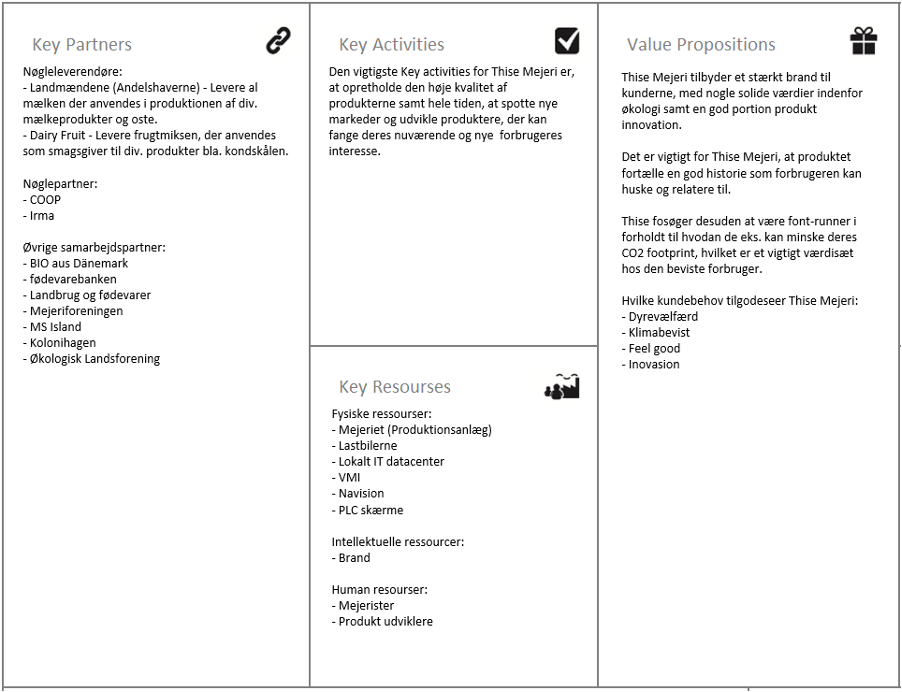
\includegraphics{images/image-1487588843.png}

Figur 2 - Alexandremodellen

\includegraphics{images/Skærmbillede 2022-12-30 kl. 10.40.26.png}

Figur 3 - Data Product Canvas

\includegraphics{images/Skærmbillede 2022-12-30 kl. 10.44.38.png}

Hypoteser fra DPC.

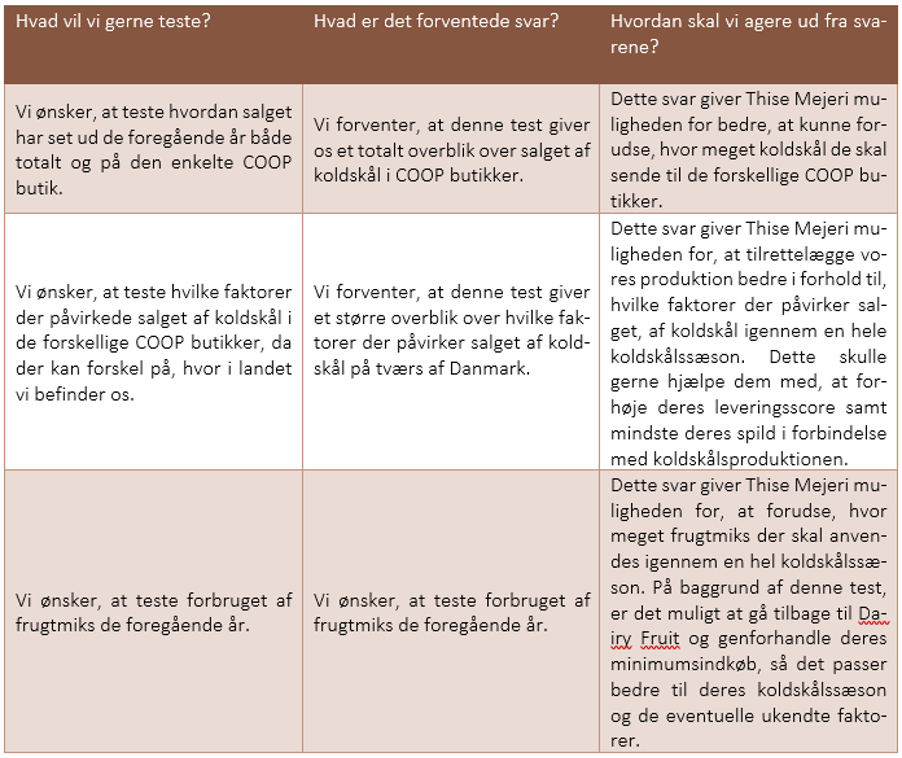
\includegraphics{images/image-198045253.png}

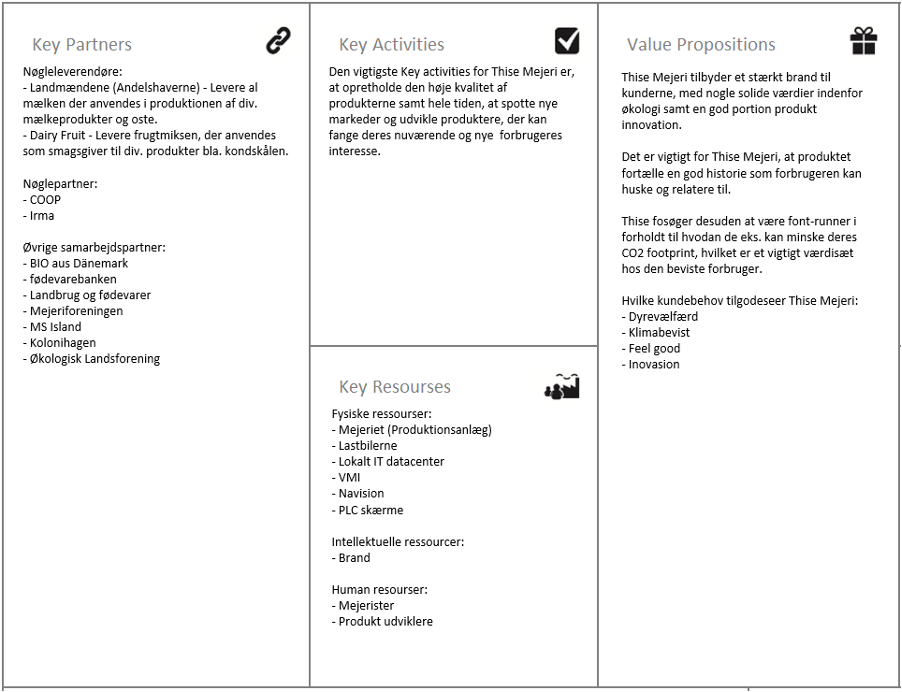
\includegraphics{images/image-481320815.png}

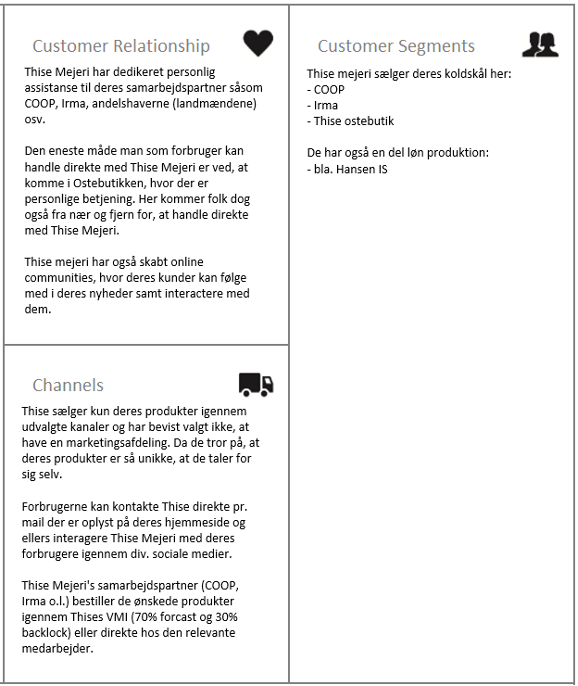
\includegraphics{images/image-1052926965.png}

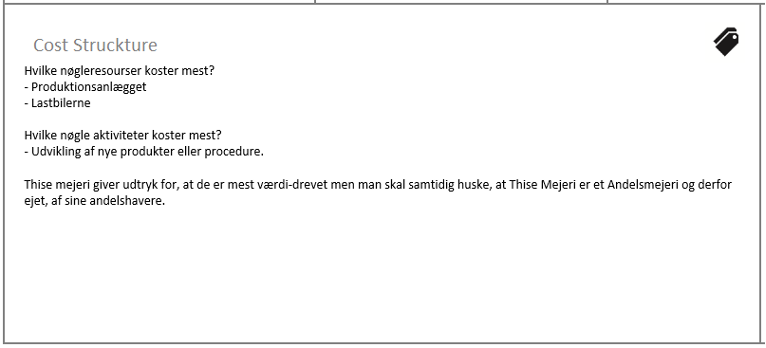
\includegraphics{images/image-878613547.png}

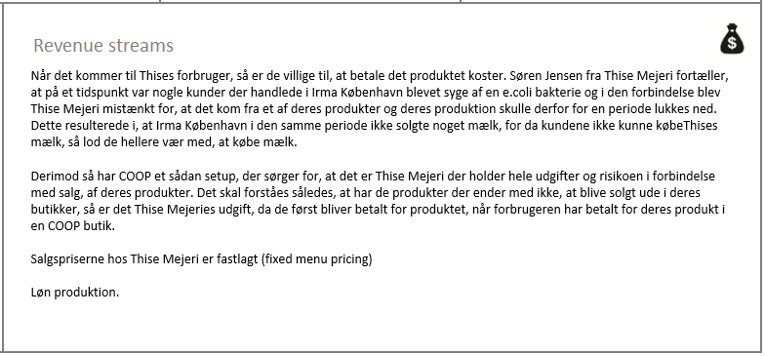
\includegraphics{images/image-735341634.png}

\includegraphics{images/Skærmbillede 2023-01-03 kl. 14.50.56.png}



\end{document}
